\documentclass[fleqn,10pt]{wlscirep}
\usepackage[utf8]{inputenc}
\usepackage[T1]{fontenc}
\usepackage{graphicx}
\usepackage{siunitx}
\usepackage{subcaption}
\usepackage{xargs}  % Use more than one optional parameter in a new commands
\usepackage[colorinlistoftodos,prependcaption]{todonotes}

\graphicspath{{figures/}}
\sisetup{locale=US,group-minimum-digits=5,group-separator={,}}

\newcommandx{\alltodo}[2][1=]{\todo[author=Everyone,linecolor=red,backgroundcolor=red!25,bordercolor=red,#1]{#2}}
\newcommandx{\mctodo}[2][1=]{\todo[author=Matt,linecolor=blue,backgroundcolor=blue!25,bordercolor=blue,#1]{#2}}
\newcommandx{\rokemtodo}[2][1=]{\todo[author=Ariel,linecolor=green,backgroundcolor=green!25,bordercolor=green,#1]{#2}}
\newcommandx{\comment}[2][1=]{\todo[author=Comment,linecolor=lime,backgroundcolor=lime!25,bordercolor=lime,#1]{#2}}
\newcommandx{\arhtodo}[2][1=]{\todo[author=Adam,linecolor=purple,backgroundcolor=purple!25,bordercolor=purple,#1]{#2}}

\title{A preprocessed open diffusion derivatives dataset for child and adolescent neuroimaging}

\author[1,*$\dagger$]{Adam Richie-Halford}
\author[2,$\dagger$]{Matthew Cieslak}
\author[4]{Lei Ai}
\author[5]{Sendy Caffarra}
\author[4]{Alexandre R. Franco}
\author[5]{Iliana Karipidis}
\author[3]{John Kruper}
\author[4]{Michael Milham}
\author[5]{Barbara Avelar Pereira}
\author[5]{Ethan Roy}
\author[2]{Valerie J. Sydnor}
\author[5]{Jason Yeatman}
\author[6]{The Fibr Community Science Consortium}
% \author[6]{Jul\_dugre}
\author[6]{amandamcgow}
\author[6]{SimonMB}
\author[6]{Nabbott}
\author[6]{AmjadSamara}
\author[6]{Shannon Grogans}
\author[6]{Zzzdeng}
\author[6]{HamidTurker}
\author[6]{Dragon}
\author[6]{Lshaffe6}
\author[6]{Hilarym}
\author[6]{faskybrain}
\author[6]{RaeYuan}
\author[6]{wanderinggrace}
\author[6]{sofie}
\author[6]{llotter}
\author[6]{valeriejill}
\author[6]{AkiNikolaidis}
\author[6]{Deagaric}
\author[6]{akoz}
\author[6]{summerf}
\author[6]{lindenmp}
\author[6]{mjl0062}
\author[6]{Nevena}
\author[6]{kat\_sh}
\author[6]{LeonF}
\author[6]{anjaue}
\author[6]{utooley1}
\author[6]{adrian\_neurosci}
\author[6]{mattwall}
\author[6]{Griffin SH}
\author[6]{jbourque}
\author[6]{averigiudicessi}
\author[6]{ncolenbi}
\author[6]{vtrip}
\author[6]{MeganHimes}
\author[6]{ti}
\author[6]{floundersmw}
\author[6]{itsyuchao}
\author[6]{jjfc}
\author[6]{Agwiesman}
\author[6]{bhaggerty}
\author[6]{benjamindeleener}
\author[6]{AnthonyJa}
\author[6]{seedyh}
\author[6]{nm\_fibr}
\author[6]{matthew2}
\author[6]{Li}
\author[6]{Gabriel Gonzalez-Escamilla}
\author[6]{Gianpaolo}
\author[6]{Mareike}
\author[6]{arielleered}
\author[6]{gdelap}
\author[6]{elliem}
\author[6]{skorenic}
\author[6]{Mark Wiesman}
\author[6]{SHKohl}
\author[6]{claudiap}
\author[6]{mackenzie}
\author[6]{jaewsong}
\author[6]{guillaume}
\author[6]{sadieneuro}
\author[6]{GuiomarNiso}
\author[6]{PSB}
\author[6]{elorenc}
\author[6]{smarek}
\author[6]{fsayed}
\author[6]{gthf61448}
\author[6]{WendyWang}
\author[6]{dcg2153}
\author[6]{mpeter55}
\author[6]{earoy}
\author[6]{cmich}
\author[6]{ikahhale}
\author[6]{czaj}
\author[6]{JodyFinch11}
\author[6]{albie}
\author[6]{holoships}
\author[6]{ckw84}
\author[6]{Gaga}
\author[6]{ecoffey}
\author[6]{jmayor}
\author[6]{jbryn}
\author[6]{jlurp20}
\author[6]{ShaoshiZ}
\author[6]{slhkam}
\author[6]{ckorponay}
\author[6]{BrunoHeblingVieira}
\author[6]{Yacine Mahdid}
\author[6]{harriet89}
\author[6]{Christian}
\author[6]{JonathanTSchneider}
\author[6]{bennewman}
\author[6]{sidchop}
\author[6]{Smeisler}
\author[6]{roryboyle}
\author[6]{cMadan}
\author[6]{MaryLena}
\author[6]{mkp}
\author[6]{Twelton}
\author[6]{dalez}
\author[6]{hyruuk}
\author[6]{ehhall}
\author[6]{jlhanson5}
\author[6]{smomara}
\author[6]{EvrenOzarslan}
\author[6]{ctw}
\author[6]{mollyr}
\author[6]{NChaku}
\author[6]{iliazaharov}
\author[6]{askeller}
\author[6]{clh64}
\author[6]{flat\_brainer}
\author[6]{H Farmer}
\author[6]{Jacobjcrouse}
\author[6]{Ryguy}
\author[6]{VincentBottom}
\author[6]{aomary}
\author[6]{aojha7}
\author[6]{wanderine}
\author[6]{Kahini}
\author[6]{bc1115}
\author[6]{adam}
\author[6]{sasims}
\author[6]{anovan}
\author[6]{patriciaschm}
\author[6]{dlsta}
\author[6]{berwe48}
\author[6]{Token Tech Chick}
\author[6]{Michael Cormican}
\author[6]{mhettwer}
\author[6]{pkirk}
\author[6]{lexlosia}
\author[6]{n00bmaster69}
\author[6]{Greki}
\author[6]{GuidoG}
\author[6]{ben}
\author[6]{yhahn1819}
\author[6]{GiuliaLiberati}
\author[6]{skyesinc}
\author[6]{djdlc85}
\author[6]{janderz8}
\author[6]{aiwiesman}
\author[6]{kurtzoner}
\author[6]{Dwin}
\author[6]{harman}
\author[2,$\ddagger$]{Theodore D. Satterthwaite}
\author[3,1,$\ddagger$]{Ariel Rokem}

\affil[1]{University of Washington, eScience Institute, Seattle, Washington, 98195, USA}
\affil[2]{University of Pennsylvania, Department of Psychiatry, Philadelphia, Pennsylvania, 19104, USA}
\affil[3]{University of Washington, Department of Psychology, Seattle, Washington, 98195, USA}
\affil[4]{Child Mind Institute, New York City, 10022, USA}
\affil[5]{Stanford University, Graduate School of Education and Division of Developmental and Behavioral Pediatrics, Stanford, California, 94305, USA}
\affil[6]{The Fibr Community Science Consortium}

\affil[*]{richford@uw.edu}
\affil[$\dagger$]{these authors contributed equally to this work}
\affil[$\ddagger$]{these authors contributed equally to this work}

%\keywords{Keyword1, Keyword2, Keyword3}

\begin{abstract}
The Healthy Brain Network (HBN) is a landmark pediatric mental health study.
Among other data, the HBN collects diffusion MRI (dMRI) from its participants,
used to make inferences about brain connections. We curated the
currently-available dMRI data from \num{2747} HBN subjects into the widely
accepted Brain Imaging Data Structure (BIDS) format, we processed the data
through a series of standard steps, to denoise the data and correct it for
motion and eddy current effects. To perform quality control (QC) on this large
dataset, we deployed a community science app. Together with a small subset of
expert QC data, community science QC scores provided the information needed to
train an artificial neural network that scores the data for quality in a manner
that highly agrees with expert QC. We demonstrate that the neural network uses
sensible features of the data and also demonstrate that accurate quality control
has implications for subsequent analysis of this data. We openly released the
processed derivatives and QC scores for use by the scientific community.
\end{abstract}

\begin{document}

\flushbottom
\maketitle
\thispagestyle{empty}

\todo[inline]{%
    Note to editing authors:

    We're targeting an eLife ``Tools and Resources'' paper for first submission,
    but we have used the Scientific Data \LaTeX template. For Scientific data,
    the abstract max is 170 words. eLife has no set max.

    We use the \texttt{todonotes} package to keep track of remaining tasks and
    comments. You can add a task for Adam with the
    \texttt{\textbackslash{}arhtodo} command, a task for Matt with the
    \texttt{\textbackslash{}mctodo} command, a task for Ariel with the
    \texttt{\textbackslash{}rokemtodo} command, a task for all reviewing authors
    with the \texttt{\textbackslash{}alltodo} command, and a general comment
    with the \texttt{\textbackslash{}comment} command.
}
\comment[inline]{Comments look like this.}
\arhtodo[inline]{Tasks for Adam look like this.}
\rokemtodo[inline]{Tasks for Ariel look like this.}
\mctodo[inline]{Tasks for Matt look like this.}
\alltodo[inline]{Tasks for all reviewing authors look like this.}

\section*{Introduction}

Childhood and adolescence are marked by rapid dynamic change to human brain
structure and function \cite{Lebel2018-oy}. It is also a time during which the
symptoms of many mental health disorders tend to emerge \cite{Paus2008-gi}.
Understanding individual differences in brain development and understanding the
interplay between brain development and the development of these disorders
requires measurements from many individuals \cite{Paus2010-qk, Fair2021-eg}.
To address this requirement, the Healthy Brain Network (HBN) is a landmark pediatric mental health study
collecting MRI images and clinical assessment data from \num{10000} New York
City area children and adolescents \cite{alexander2017-yc}. The HBN dataset
takes a trans-diagnostic approach, measuring a broad range of phenotypic and
imaging data in each individual. One of the brain imaging measurements conducted
in every individual is diffusion MRI (dMRI), which allows for analysis of the
physical properties of developing white matter \cite{wandell2016-qt}. The dMRI
data is openly available in its raw form through the Functional Connectomes
Project and the International Neuroimaging Data-Sharing Initiative (FCP-INDI),
spurring collaboration on open big-data reproducible science
\cite{avesani2019-ey}. However, even with the data publicly available, several
steps need to be completed before the data can be fruitfully analyzed.

First, analysis of dMRI data must start with a pipeline of critical
preprocessing steps, such as eddy current correction, motion correction, and
adjustment of the gradient directions. Because of the complexity of some of
these steps, investigators may neglect to perform some preprocessing steps or
may make errors that can induce bias in their subsequent interpretation of the
data \cite{jones2010-ps}. Furthermore, once preprocessing is done correctly and
transparently once, there is little need for researchers to repeat this step.
Thus, there is a need for an openly available preprocessed diffusion derivative
dataset that applies best practices in preprocessing in a robust and transparent
way. Here, we used \emph{QSIPrep}, an integrative platform for preprocessing and
reconstructing diffusion MRI data, which implements these best practices
\cite{cieslak2021-iq}. To find the relevant files within a dataset, \emph{QSIPrep}
relies on the Brain Imaging Data Specification (BIDS) standard
\cite{gorgolewski2016-lh}, which describes the way to organize neuroimaging data
for automated processing. That is, it is a BIDS App \cite{Gorgolewski2017-mb}.
To reach full compliance with the BIDS standard, data in HBN had to first be
curated.

\mctodo[inline]{maybe we need a couple more words here to say what that means?}

Second, dMRI measurements are susceptible to a variety of artifacts that affect
the quality of the signals and the ability to make accurate inferences from
them. In small studies, with few participants, it is common to thoroughly
examine the data from every participant as part of a quality control (QC)
process. Expert examination is time consuming and is prohibitive in large
datasets, such as HBN. This difficulty could be ameliorated through the
automation of QC. Thanks to their success in many other visual recognition
tasks, previously only achievable by humans, machine learning and computer
vision methods, such as convolutional deep artificial neural networks, or ``deep
learning'' \cite{lecun2015deep} are promising avenues for automation of QC. One
of the challenges of these new methods is that they require a large training
dataset to attain accurate performance. In previous work, we demonstrated that
deep learning can accurately emulate expert examination of T1-weighted
(T1w)brain images for QC \cite{keshavan2019-er}. To obtain a large enough
training dataset of T1w images in that case, we deployed a community science
application that collected quality control scores of parts of the dataset from
volunteers through a web application \footnote{%
    While the legacy term ``citizen science'' evokes a sense of civic duty in
    scientific engagement, it can also imply a barrier for community members who
    want to contribute to science but may not be citizens of a particular
    country. In this manuscript we use the more modern term ``community
    science.''
}.
These scores were then calibrated using a gold standard expert-scored subset of
these images. A deep learning neural network was trained on the calibrated and
aggregated score, resulting in very high concordance with expert ratings on a
separate test dataset. We term this approach ``hybrid QC'', because it combines
information from experts with information from community scientists to create a
scalable machine learning algorithm that can be applied to future data
collection.

However, the hybrid QC proof-of-concept left lingering questions about its
applicability to other datasets because it was trained on a single-site,
single-modality dataset. Here, we expand the hybrid-QC approach to a large
multi-site diffusion MRI dataset. Moreover, one of the common critiques of deep
learning is that it can learn irrelevant features of the data and does not
provide information that is transparent enough to interpret
\cite{lipton2017doctor, salahuddin2022transparency, Zech2018-ki}. To confirm
that the hybrid-QC deep learning algorithm uses meaningful features of the
diffusion-weighted images to perform accurate QC, we used machine learning
interpretation methods that pry open the ``black box'' of the neural network
highlighting the features that lead to a specific QC score
\cite{sundararajan2017axiomatic,murdoch2019definitions}.

Taken together, BIDS-curated data, processed data, and quality control scores
generated by the deep learning algorithm provide researchers with everything
that they need in order to start applying a large variety of analysis approaches
to these HBN Preprocessed Open Diffusion Derivatives (HBN-POD2), and answer the
questions that this data was collected to answer.

\section*{Results}

The aims of this study were fourfold
\begin{enumerate*}[%
    label=(\roman*),%
    before=\unskip{: },%
    itemjoin={{, }},%
    itemjoin*={{, and }}]
    \item curate the HBN MRI data into a fully-BIDS compliant MRI dataset
    \item perform state-of-the-art diffusion MRI (dMRI) preprocessing using \emph{QSIPrep}
    \item assign QC scores to each subject
    \item provide unrestricted public release of the outputs from each of these
    steps.
\end{enumerate*}
Starting with MRI data from \num{2747} HBN participants available on FCP-INDI,
we curated these data for compliance with the Brain Imaging Data Structure
(BIDS) specification \cite{gorgolewski2016-lh} and preprocessed the structural
MRI (sMRI) and diffusion MRI (dMRI) data using \emph{QSIPrep}. Subjects that
could not be curated to comply with the BIDS standard or that did not have dMRI
data were excluded, resulting in \num{2136} subjects with preprocessed,
BIDS-compliant dMRI data (Figure~\ref{fig:hbn-sankey}).

\subsection*{Healthy Brain Network Preprocessed Open Diffusion Derivatives}

\mctodo[inline]{%
    Matt, please describe the \emph{QSIPrep} output directory structure.
    Maybe we include a \texttt{tree} output figure and then a description of
    each output file.
    Hint: Use \href{https://github.com/emad-elsaid/dirtree}{dirtree} to make a
    nice figure of \texttt{tree} output.
}

\arhtodo[inline]{%
    Describe the distributions of \emph{QSIPrep} automated QC metrics:
    NDC, max rel translation, raw number outlier slices.
    e.g. \texttt{sns.pairplot()} of these three, lower tri, colored by age.
}

\begin{figure}[ht]
    \centering
    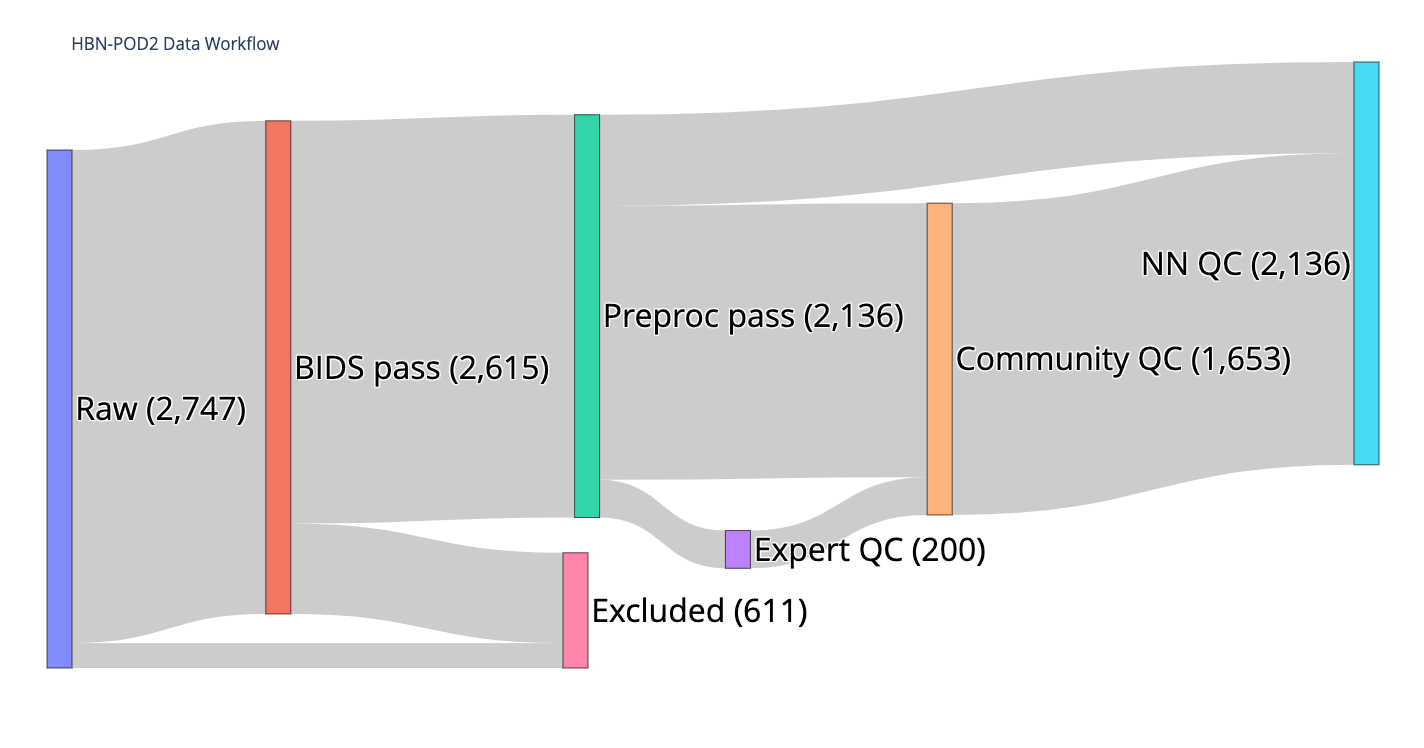
\includegraphics[width=0.75\linewidth]{hbn-pod2-sankey.png}
    \caption{%
        {\bf HBN-POD2 data provenance}:
        Imaging data for \num{2747} subjects, aged 5-21 years and collected at four
        sites in the New York City area, was made available through the
        Functional Connectomes Project and the International Neuroimaging
        Data-Sharing Initiative (FCP-INDI).
        %
        These data were curated for compliance to the BIDS specification
        \cite{gorgolewski2016-lh} and availability of imaging metadata in json
        format. \num{2615} subjects met this specification.
        %
        Imaging data was preprocessed using \emph{QSIPrep} \cite{cieslak2021-iq}
        to group, distortion correct, motion correct, denoise, coregister and
        resample MRI scans. Of the BIDS curated subjects, \num{2136} subjects
        passed this step, with the majority of failures coming from subjects
        with missing dMRI scans.
        %
        Expert raters assigned QC scores to \num{200} of these participants,
        creating a ``gold standard'' QC subset. Community raters then assigned
        binary QC ratings to a superset of the gold standard containing
        \num{1653} participants. An image classification algorithm was trained
        on a combination of automated QC metrics from \emph{QSIPrep} and community
        scientist reviews to ``extend'' the expert ratings to the community
        science subset. Finally, a deep learning QC model was trained on the
        community science subset to assign QC scores to the entire dataset and
        to future releases from HBN.
        %
        The HBN-POD2 dataset, including QC ratings, is openly available through
        FCP-INDI.
    }
    \label{fig:hbn-sankey}
\end{figure}

\subsection*{Quality Control}

To achieve the QC aim of the project, we adopted a hybrid QC approach that
combines expert rating, community science, and deep learning, drawing on the
success of a previous application in assessing the quality of HBN's structural
MRI data \cite{keshavan2019-er}. This method
\begin{enumerate*}[%
    label=(\roman*),%
    before={{ }},%
    itemjoin={{, }},%
    itemjoin*={{ and }}]
    \item starts with dMRI expert raters labelling a small subset of subjects,
    the ``gold standard'' dataset
    \item amplifies these labels using a community science web application to
    extend expert ratings to a much larger subset of the data, the community
    science subset
    \item trains a deep learning model on the community science subset to
    predict expert decisions on the entire dataset.
\end{enumerate*}

\subsubsection*{Expert quality control}

To create a gold standard QC dataset, we first developed \emph{dmriprep-viewer},
a dMRI data viewer and QC rating web application to display \emph{QSIPrep}
outputs and collect expert ratings \cite{richie-halford2021-viewer}. Six of the
co-authors, who are all dMRI experts, rated a 200-participant subset of the
HBN-POD2 data using extensive visual examination of each subjects dMRI data,
including the diffusion weighting imaging (DWI) time series itself, a plot of
motion parameters through the DWI scan, and full 3D volumes depicting
\begin{enumerate*}[%
    label=(\roman*),%
    before={{ }},%
    itemjoin={{, }},%
    itemjoin*={{ and }}]
    \item the brain mask and $b=0$ to T1w registration
    \item a directionally encoded color FA (DEC-FA) image laid over the $b=0$ volume.
\end{enumerate*}
The experts rated subjects using a five-point scale with ratings of ``definitely
fail,'' ``probably fail,'' ``unsure,'' ``probably pass,'' and ``definitely
pass.'' The distribution of scores given by the experts demonstrates that the
gold standard dataset included a range of data quality. Mean expert ratings
correlate with some of the automated QC metrics output by \emph{QSIPrep}:
neighboring DWI correlation (NDC) \cite{yeh2019-kb}, maximum relative
translation, and number of outlier slices. NDC characterizes
the pairwise spatial correlation between pairs of DWI volumes that sample
neighboring points in $q$-space. Since lower values indicate reduced data
quality, it is reassuring that NDC correlates directly with expert rating
(Pearson CC: XXX). Conversely, high relative translation and a high number of
motion outlier slices reflect poor data quality and these metrics are inversely
related to mean expert rating (Pearson CC: XXX and Pearson CC: XXX,
respectively).

\arhtodo[inline]{Fill in the XXX values in the paragraph above.}

In addition to agreeing qualitatively with \emph{QSIPrep}'s automated QC metrics
on average, the expert raters also tended to agree with each other. We assessed
inter-rater reliability (IRR) using the pairwise Cohen's $\kappa$
\cite{di-eugenio2004-bb}, which exceeds 0.52 in all cases, and with a mean value of
0.648. In addition to the pairwise Cohen's $\kappa$, we also computed the
intra-class correlation (ICC) \cite{hallgren2012-ze} as a measure of IRR. ICC3k
is the appropriate variant of the ICC to use when a fixed set of $k$ raters each
code an identical set of subjects, as is the case here. ICC3k for inter-rater
reliability among the experts was 0.930 (95\% CI: [0.91, 0.94]), which is
qualitatively considered an ``excellent'' level of IRR \cite{Cicchetti1994-fz}.
The high IRR provides confidence that the average of the expert ratings for each
image in the gold standard is an appropriate target to use for training a
machine learning model that predicts the expert scores.

\begin{figure}[ht]
    \begin{subfigure}{.5\textwidth}
    \centering
    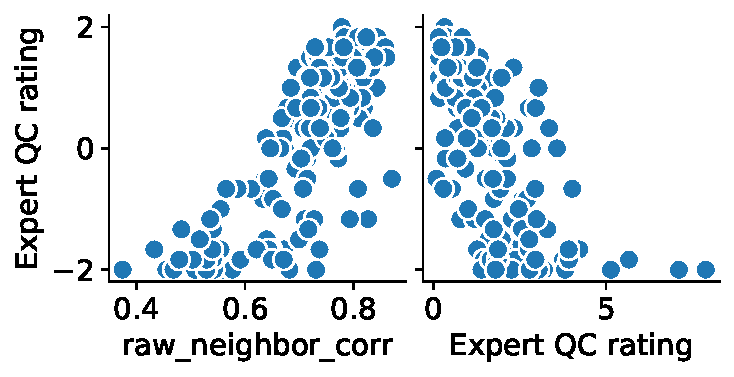
\includegraphics[width=\linewidth]{community-qc/expert-qsiprep-pairplot-top.pdf}
    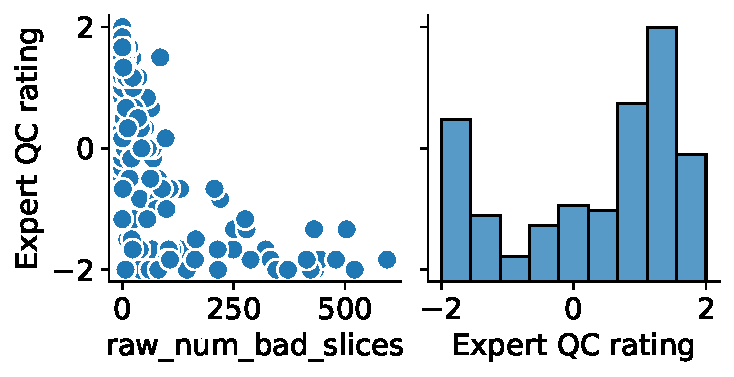
\includegraphics[width=\linewidth]{community-qc/expert-qsiprep-pairplot-bottom.pdf}
    \caption{}
    \label{fig:expert-qc:scatter}
    \end{subfigure}
    \begin{subfigure}{.5\textwidth}
    \centering
    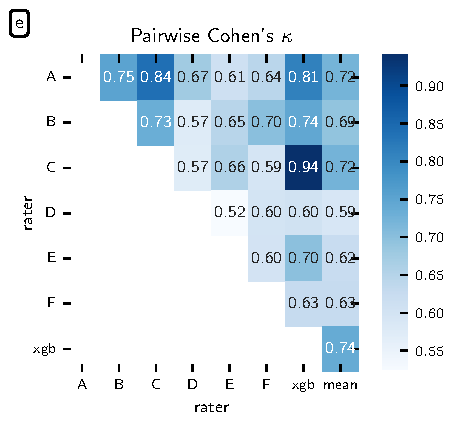
\includegraphics[width=\linewidth]{community-qc/expert-raters-cohens-kappa.pdf}
    \caption{}
    \label{fig:expert-qc:irr}
    \end{subfigure}
    \caption{%
        {\bf Expert QC results}:
        Six dMRI experts rated a subset of \num{200} subjects.
        \textbf{(a)} Experts agree with \emph{QSIPrep}'s automated QC metrics.
        Here we show associations between the expert QC rating and the
        \emph{QSIPrep} metrics neighboring diffusion-weighted imaging
        correlation (NDC) \cite{yeh2019-kb}, maximum relative translation, and
        number of outlier slices. As expected, NDC is directly correlated with expert rating while
        the other two metrics are inversely correlated with expert rating.
        %
        \textbf{(b)} Experts agree with each other. Here we show the pairwise
        Cohen's $\kappa$ measure of inter-rater reliability (see text for ICC
        calculations). The XGB model has an inter-rater reliability (quantified
        here as Cohen's $\kappa$) that is indistinguishable from the other
        raters
    }
    \label{fig:expert-qc}
\end{figure}

\subsubsection*{Community science quality control}

Although the expert raters achieved high IRR and yielded intuitive associations
with \emph{QSIPrep}'s automated QC metrics, generating expert QC labels for the
entire HBN-POD2 dataset would be prohibitively time consuming. To assess the
image quality of the remaining subjects, we deployed \emph{Fibr}
(\url{https://fibr.dev}), a community science web application in which users
assign binary pass/fail labels assessing the quality of horizontal slice DEC-FA
images overlaid on the $b=0$ image. That is, \emph{Fibr} users saw individual
slices or an animated sequence of ten slices taken from the entire DEC-FA volume
that the expert raters saw. The \emph{Fibr} users therefore saw only a subset of
the imaging data that the dMRI experts had access to for each subject, but they
saw many more subjects. In total, \num{374} community scientists provided
\num{587778} ratings for a mean of $>50$ ratings per slice (or $>200$ ratings
per subject) from \num{1653} subjects. Of the community scientists, \num{145}
raters provided $>3,000$ ratings each and are included in the Fibr Community
Science Consortium as co-authors on this paper.

The unadjusted \emph{Fibr} ratings are overly optimistic; i.e., on average,
community scientists are not as critical as the expert raters
(Figure~\ref{fig:fibr-qc:scatter}a). In addition, different community scientists
probably provide data of differing accuracy. In addition, additional information
about quality is provided in the \emph{QSIPrep} QC metrics. To account for this
variability, and take advantage of the information provided by \emph{QSIPrep},
we trained a gradient boosting model \cite{chen2016-eb} to predict expert scores
based on a combination of community science ratings and automated \emph{QSIPrep}
QC metrics. We refer to this model as XGB.

To clarify the contributions of the automated QC metrics and the community
science raters, we trained two additional gradient boosting models
\begin{enumerate*}[%
    label=(\roman*),%
    before=\unskip{: },%
    itemjoin={{, }},%
    itemjoin*={{ and }}]
    \item one trained only on the automated \emph{QSIPrep} QC metrics, which we
    call XGB-q
    \item one trained on only the \emph{Fibr} ratings, which we call XGB-f.
\end{enumerate*}
XGB-f may be viewed as a data-driven weighting of community scientists' ratings,
while XGB-q may be viewed as a generalization of QC metric exclusion criteria.
XGB, combining information from both \emph{Fibr} ratings and \emph{QSIPrep} QC
metric attained a cross-validated area under the receiver operating curve
(ROC-AUC) of $0.96 \pm 0.01$ on the ``gold standard,'' where the $\pm$ indicates
the standard deviation of scores from repeated $k$-fold cross-validation
(Figure~\ref{fig:fibr-qc:scatter}a). In contrast, XGB-q attained an ROC-AUC of
$0.91 \pm 0.03$ and XGB-f achieved an ROC-AUC of $0.84 \pm 0.04$. The enhanced
performance of XGB-q over XGB-f shows that community scientists alone are not as
accurate as automated QC metrics are at predicting expert ratings. And yet, the
increased performance of XGB over XGB-q demonstrates that there is additional
image quality information to be gained by incorporating community scientist input.

As a way of evaluating the quality of the XGB predictions, consider the fact
that the average Cohen's $kappa$ between XGB and the expert raters is 0.74,
which is higher than the average Cohen's $kappa$ between any of the other raters
and their human peers (Figure~\ref{fig:expert-qc}). This is not suprising,
given that the XGB model was fit to optimize this match, but further
demonstrates the goodness of fit of this model.

Nevertheless, this provides confidence in using the XGB scores in the next step
of analysis. When a subset of subjects is coded by multiple raters and the
reliability of their ratings is meant to generalize to other subjects rated by
only one coder, the single-measure ICC3 must be used. When adding XGB to the
existing expert raters as a seventh expert, $\textbf{ICC3} = 0.709 (95\% CI:
[0.66, 0.75])$. This high ICC3 value after inclusion of the XGB model justifies
using the XGB scores as the target for training an image-based deep learning
network.

\begin{figure}[tbp]
    \begin{subfigure}{.55\textwidth}
    \centering
    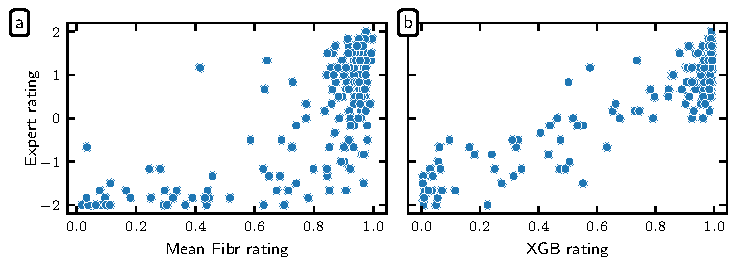
\includegraphics[width=\linewidth]{community-qc/fibr-rating-scatter-plot.pdf}
    \caption{}
    \label{fig:fibr-qc:scatter}
    \end{subfigure}
    \begin{subfigure}{.45\textwidth}
    \centering
    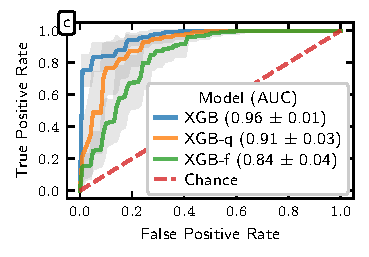
\includegraphics[width=\linewidth]{community-qc/xgb-roc-curve.pdf}
    \caption{}
    \label{fig:fibr-qc:roc}
    \end{subfigure}
    \caption{%
        {\bf Community science predictions of the expert ratings}:
        \textbf{(a)} Scatterplots showing the relationship between mean expert
        rating and both mean \emph{Fibr} rating (left) and XGB prediction
        (right). \emph{Fibr} raters overestimate the quality of images compared
        to expert raters. But the XGB prediction compensates for this by
        incorporating automated QC metrics and weighting more valuable
        \emph{Fibr} raters.
        %
        \textbf{(b)} ROC curves for the XGB, XGB-q, and XGB-f models.
        Transluscent bands represent one standard deviation from the mean
        of the cross-validation splits.
    }
    \label{fig:fibr-qc}
\end{figure}

\subsubsection*{Automated quality control labelling through deep learning}

The XGB ``rater'' does a good job of extending QC ratings to the entire
community science subset, but requires \emph{Fibr} scores. Without community
science ratings, we would have to fall back on the less accurate XGB-q
prediction. Instead, we would like a fully automated QC approach that can be
readily applied to new data releases from HBN.

We therefore trained a deep convolutional neural network to predict the XGB
ratings directly from \emph{QSIPrep} outputs. We modified an existing 3D
convolutional neural network (CNN) architecture \cite{zunair2020-bs}, previously
applied to the ImageCLEF Tuberculosis Severity Assessment 2019 benchmark
\cite{dicente2019clef} to accept multichannel input generated from the
preprocessed dMRI: the $b=0$ reference diffusion image, each of the three
cardinal axis components of the DEC-FA image, and, optionally, automated QC
metrics from \emph{QSIPrep}. We trained this network on XGB scores and validated it
against the gold standard expert-scored dataset. We refer to the convolutional
neural network model trained only on imaging data as CNN-i and the model that
incorporates automated QC metrics as CNN-i+q. The two models performed nearly
identically and achieved an ROC-AUC of $0.947$ (Figure~\ref{fig:dl-qc:roc}). The
near-identical performance suggests that \emph{QSIPrep}'s automated QC metrics
provide information that is redundant with information available in the imaging
data. Both CNN-i and CNN-i+q outperformed XGB-q, which was trained only on
automated QC metrics, but both underperformed relative to the full XGB model,
that uses \emph{Fibr} scores in addition to the \emph{QSIPrep} QC scores.

\begin{figure}[htbp]
    \begin{subfigure}{.25\textwidth}
    \centering
    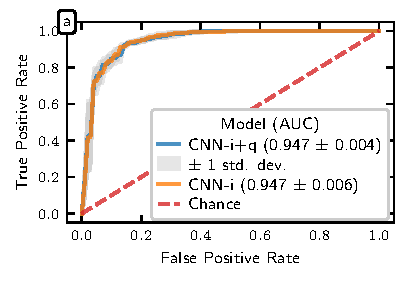
\includegraphics[width=\linewidth]{deep-learning-qc/dl_roc_auc_curve.pdf}
    \caption{}
    \label{fig:dl-qc:roc}
    \end{subfigure}
    \begin{subfigure}{.25\textwidth}
    \centering
    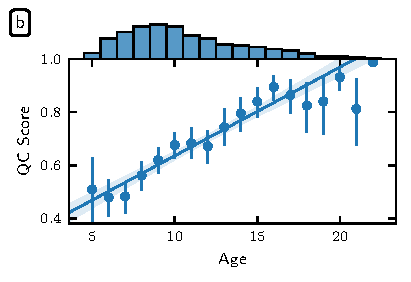
\includegraphics[width=\linewidth]{bundle-profiles/qc-age-jointplot.pdf}
    \caption{}
    \label{fig:dl-qc:joint}
    \end{subfigure}
    \begin{subfigure}{.5\textwidth}
    \centering
    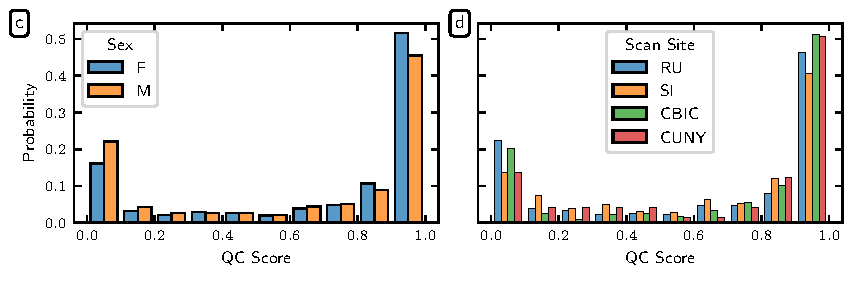
\includegraphics[width=\linewidth]{bundle-profiles/qc-hist.pdf}
    \caption{}
    \label{fig:dl-qc:hist}
    \end{subfigure}
    \caption{%
        {\bf Deep learning QC scores}:
        \textbf{(a)} ROC curves for two deep learning models: one trained with
        additional automated QC metrics from \emph{QSIPrep} (blue) and one
        trained without (orange). The models performed roughly identically,
        indicating the the QC metrics provide information that is redundant to
        the imaging. Both outperformed the XGB-q predictions, indicating the
        added value of the diffusion weighted images. However, both models
        underperformed the XGB predictions, which also incoporate
        information from \emph{Fibr} ratings for each scan. The error bands
        represent one standard deviation from the mean of the cross-validation
        splits.
        %
        \textbf{(b)} Joint distributions showing a strong direct association
        between age and QC score. This likely reflects the well-known negative
        association between age and head motion in pediatric neuroimaging.
        The dots encode the mean QC score for each year of age with error bands
        representing a bootstrapped 95\% confidence interval. The line depicts
        a linear regression relating age and QC score with transluscent bands
        encoding a bootstrapped 95\% confidence interval.
        %
        \textbf{(c)}
        Histograms showing the relationship between participants QC scores and
        their sex (left) and scan site (right). QC distributions are independent
        of sex and scanning site
    }
    \label{fig:dl-qc}
\end{figure}

While HBN-POD2 provides four QC ratings: the mean expert QC ratings, XGB-q and
XGB predicted scores, as well as the CNN-i predicted score, we treat the CNN-i
score as the definitive QC score because it is available for all participants,
can be easily calculated for new participants in future HBN releases and is more
accurate than XGB-q. When we refer to a participant's QC score without
specifying a generating model, the CNN-i score is assumed.
Figure~\ref{fig:dl-qc} depicts the distribution of these QC scores by age
(Figure~\ref{fig:dl-qc:joint}), sex, and scanning site
(Figure~\ref{fig:dl-qc:hist}). QC distributions are similar for each scan site
and for male and female participants \footnote{%
    Responses for the sex variable in HBN phenotypic data are limited to
    ``male'' and ``female.''
}.

\subsubsection*{Attribution masks for the deep learning classifier}

We generated post-hoc attribution maps that highlight regions of the input
volume that are relevant for the QC score. The integrated gradient method
\cite{sundararajan2017axiomatic} is a gradient-based attribution method
\cite{ancona2019gradient} that aggregates gradients for synthetic images
interpolating between a baseline image and the input image. It has been used to
interpret deep learning models applied to retinal imaging in diabetic
retinopathy \cite{sayres2019using} and glaucoma \cite{Mehta2021-zp} prediction,
as well as in multiple sclerosis prediction from brain MRI
\cite{wargnier-dauchelle2021interpretable}. Our goal is to confirm that the
CNN-i model is looking at the same features that an expert rater would look at,
thereby bolstering the decision to apply it to new data.

Figure~\ref{fig:ig} shows attribution maps for example participants from each
confusion class: true positive, true negative, false positive, and false
negative. The columns correspond to the different channels of the deep learning
input volume: the $b=0$ reference image and the DEC-FA in the $x$, $y$, and $z$
directions. The true positive map indicates that the network is looking at the
entire brain rather than focusing on any one anatomical region
(Figure~\ref{fig:ig:true-pos}). Moreover, the model identifies white matter
fascicles that travel along the direction of the input channel: lateral for $x$,
anterior-posterior for $y$, and superior-inferior for $z$. The true negative
attribution map (Figure~\ref{fig:ig:true-neg}) reveals that when the reference
$b=0$ volume contains motion artifacts, such as banding, the network ignores the
otherwise positive attributions for the clearly identifiable white matter tracts
in the DEC-FA channels. The false positive map (Figure~\ref{fig:ig:false-pos})
and the false negative map (Figure~\ref{fig:ig:false-neg}) should be interpreted
differently since they come from low confidence predictions; the probability of
passing hovered on either side of the pass/fail threshold. For example, in the
false positive case, the network is confused enough that it treats voxels that
are outside of the brain as informative as voxels in the major white matter
bundles.

\begin{figure}[tbp]
    \centering
    \begin{subfigure}{\textwidth}
    \centering
    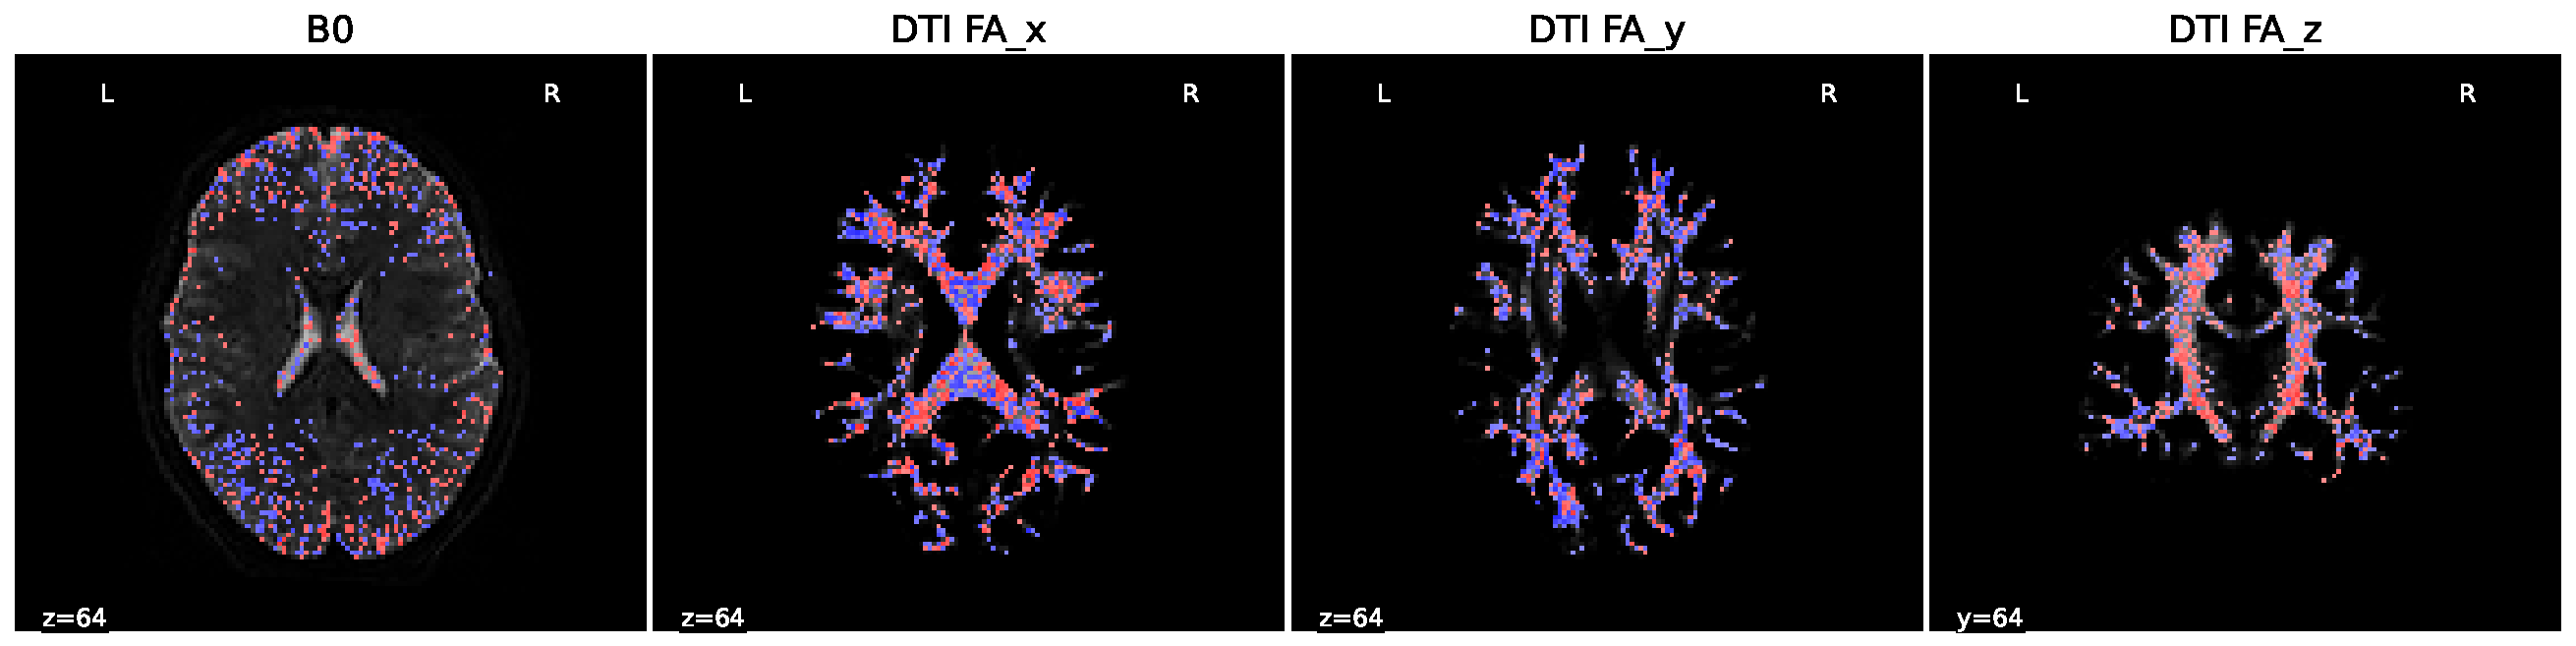
\includegraphics[width=0.9\linewidth]{deep-learning-qc/attribution-maps-true-pos.pdf}
    \caption{true positive}
    \label{fig:ig:true-pos}
    \end{subfigure}
    \begin{subfigure}{\textwidth}
    \centering
    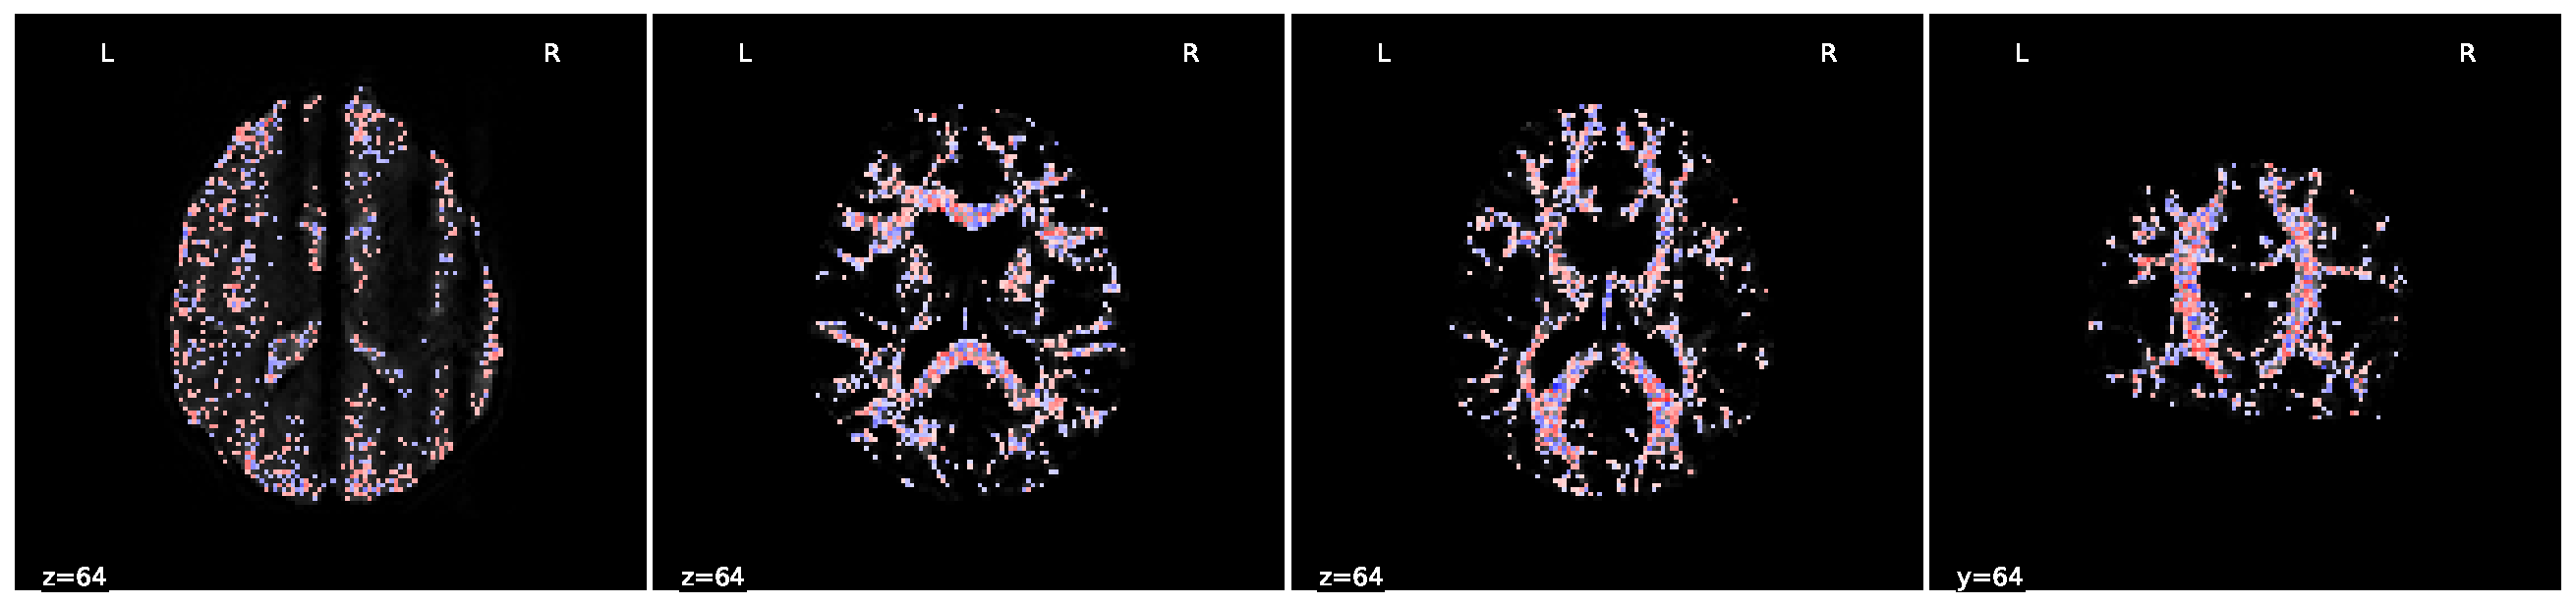
\includegraphics[width=0.9\linewidth]{deep-learning-qc/attribution-maps-true-neg.pdf}
    \caption{true negative}
    \label{fig:ig:true-neg}
    \end{subfigure}
    \begin{subfigure}{\textwidth}
    \centering
    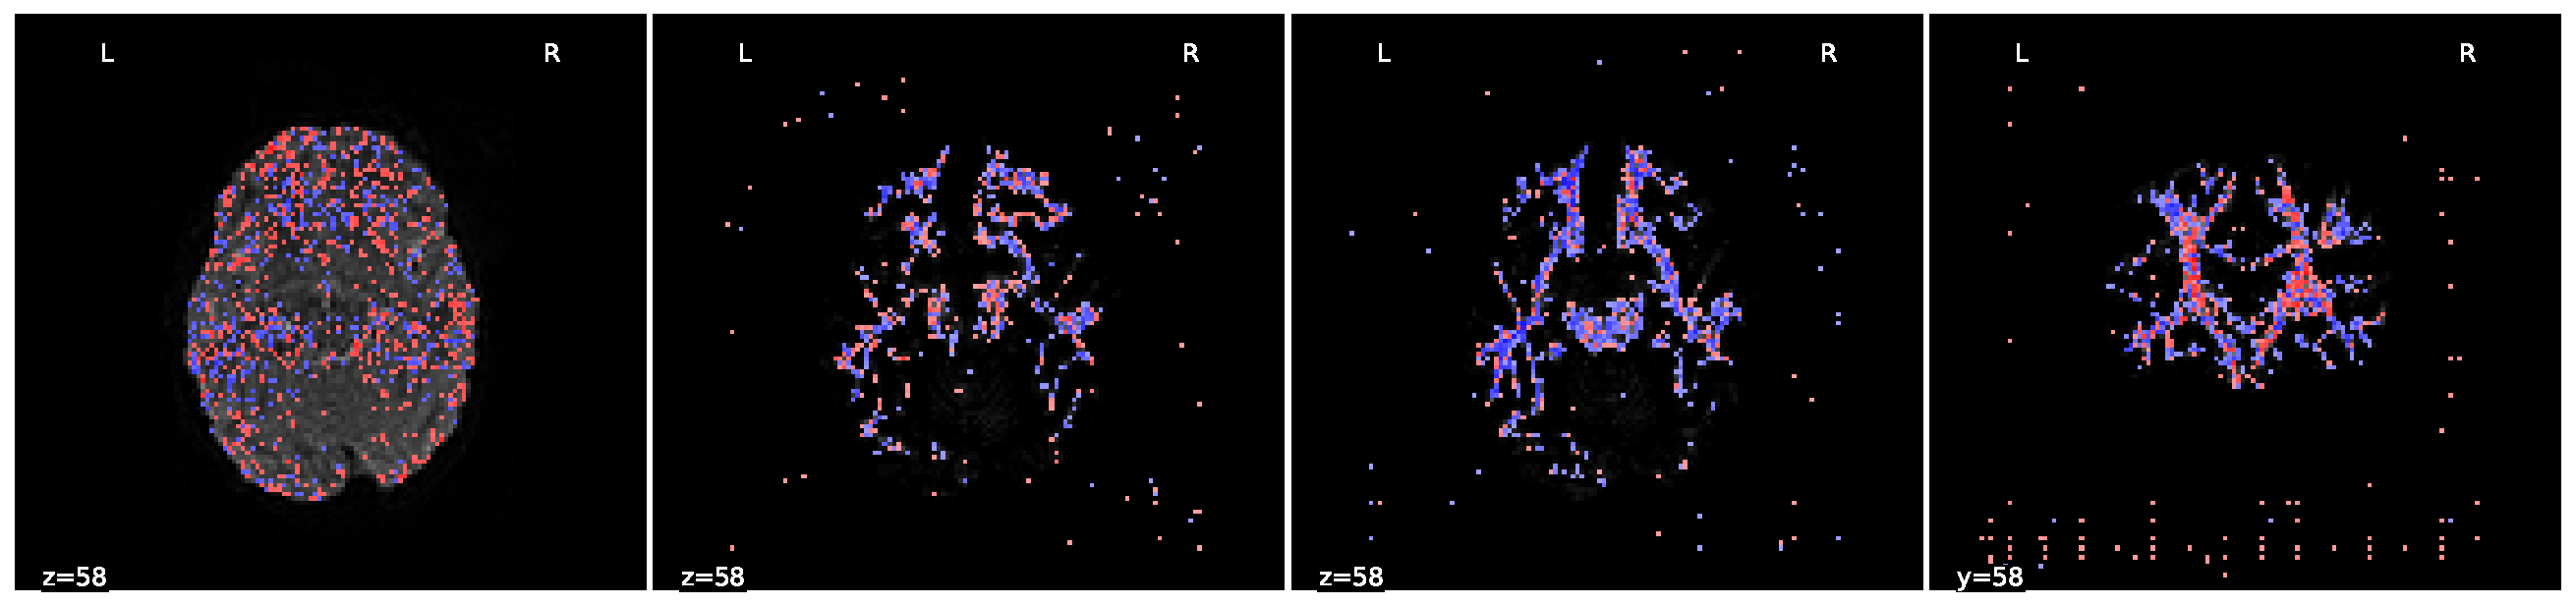
\includegraphics[width=0.9\linewidth]{deep-learning-qc/attribution-maps-false-pos.pdf}
    \caption{false positive}
    \label{fig:ig:false-pos}
    \end{subfigure}
    \begin{subfigure}{\textwidth}
    \centering
    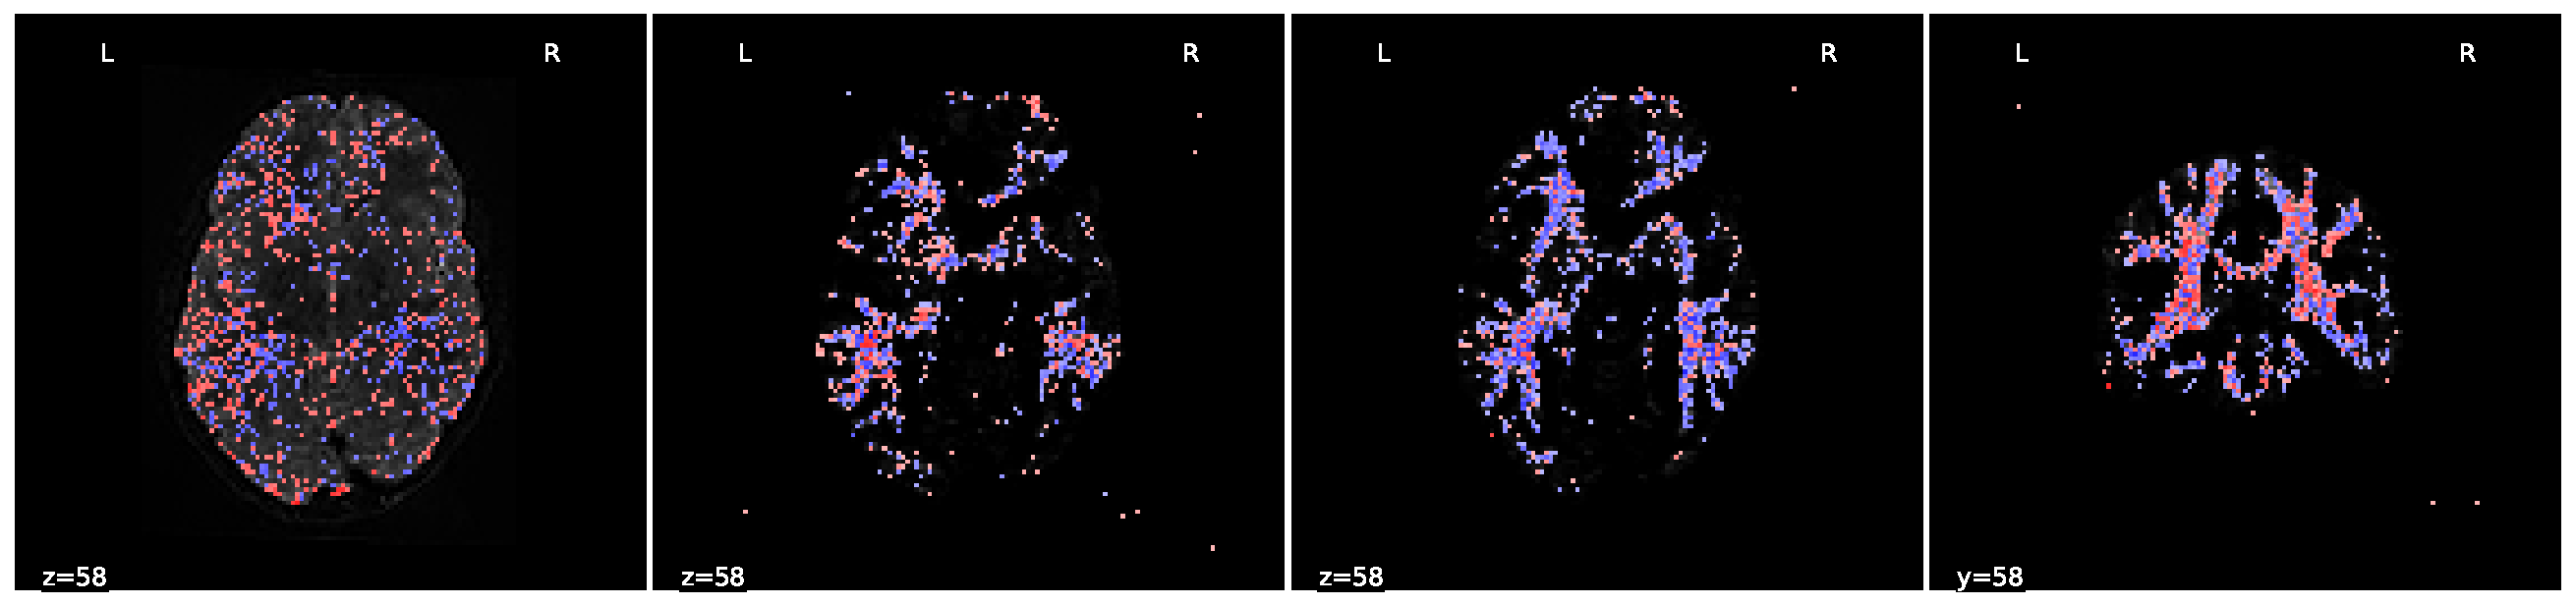
\includegraphics[width=0.9\linewidth]{deep-learning-qc/attribution-maps-false-neg.pdf}
    \caption{false negative}
    \label{fig:ig:false-neg}
    \end{subfigure}
    \caption{%
        {\bf Integrated gradients attribution maps for the deep learning classifier}:
        Each column depicts a different channel of the input tensor: the $b=0$
        DWI volume and the DEC-FA images in the $x$, $y$, and $z$ directions.
        The first three columns show a horizontal slice while the last column
        shows a coronal slice. Blue voxels indicate positive attribution (i.e.
        evidence for passing the subject), while red voxels indicate negative
        attribution (i.e. evidence for QC failure). The underlying greyscale
        depicts the input channel. Each row depicts a representative subject
        from each confusion class:
        %
        \textbf{(a)} Attribution maps for a true positive prediction. The model
        looks at the entire brain and focuses on known white matter bundles in
        the DEC-FA channels. In particular, it focuses on lateral bundles in the
        $x$ direction, anterior-posterior bundles in the $y$ direction, and
        superior-inferior bundles in the $z$ direction.
        %
        \textbf{(b)} Attribution maps for a true negative prediction. The model
        focuses primarily on the $b=0$ channel, suggesting that it ignores
        DEC-FA when motion artifacts like banding are present.
        %
        \textbf{(c)} Attribution maps for a false positive prediction. Both the
        false positive and negative predictions were low confidence predictions.
        This is reinforced by the fact that the model views some voxels that are
        outside of the brain as just as informative as those in major white
        matter tracts.
        %
        \textbf{(d)} Attribution maps for a false negative prediction. The model
        fails to find long-range white matter tracts in the anterior-posterior
        and lateral directions. We also speculate that the model expects
        left-right symmetry in the DEC-FA channels and assigns negative
        attribution to asymmetrical features. }
    \label{fig:ig}
\end{figure}

\subsection*{Quality control improves inference}

To demonstrate the effect that quality control has on inference, we analyzed
tract profile data derived from HBN-POD2 data. Tract profiling
\cite{yeatman2012-rc,jones2005pasta,colby2012along,odonnell2009tract,
kruper2021evaluating} is a subset of tractometry
\cite{jones2005pasta,bells2011tractometry}, which uses the results of dMRI
tractography to quantify properties of the white matter along major pathways.
Tract-profiling retains the values of diffusion metrics along the trajectory of
each bundle of tractography streamlines, rather than computing summary
statistics summarized at the level of each bundle. In
Figure~\ref{fig:qc-profiles:md}, we plot mean diffusivity tract profiles grouped
into four QC bins along the length of twenty-four bundles: While some bundles,
such as the cingulum cingulate (CGC) and the inferior longitudinal fasciculus
(ILF), appear insensitive to QC score, others, such as the uncinate (UNC) and
the orbital portion of the corpus callosum, exhibit strong differences between
QC bins. In most bundles, low QC scores tend to flatten the profile.

\begin{figure}[tbp]
    \centering
    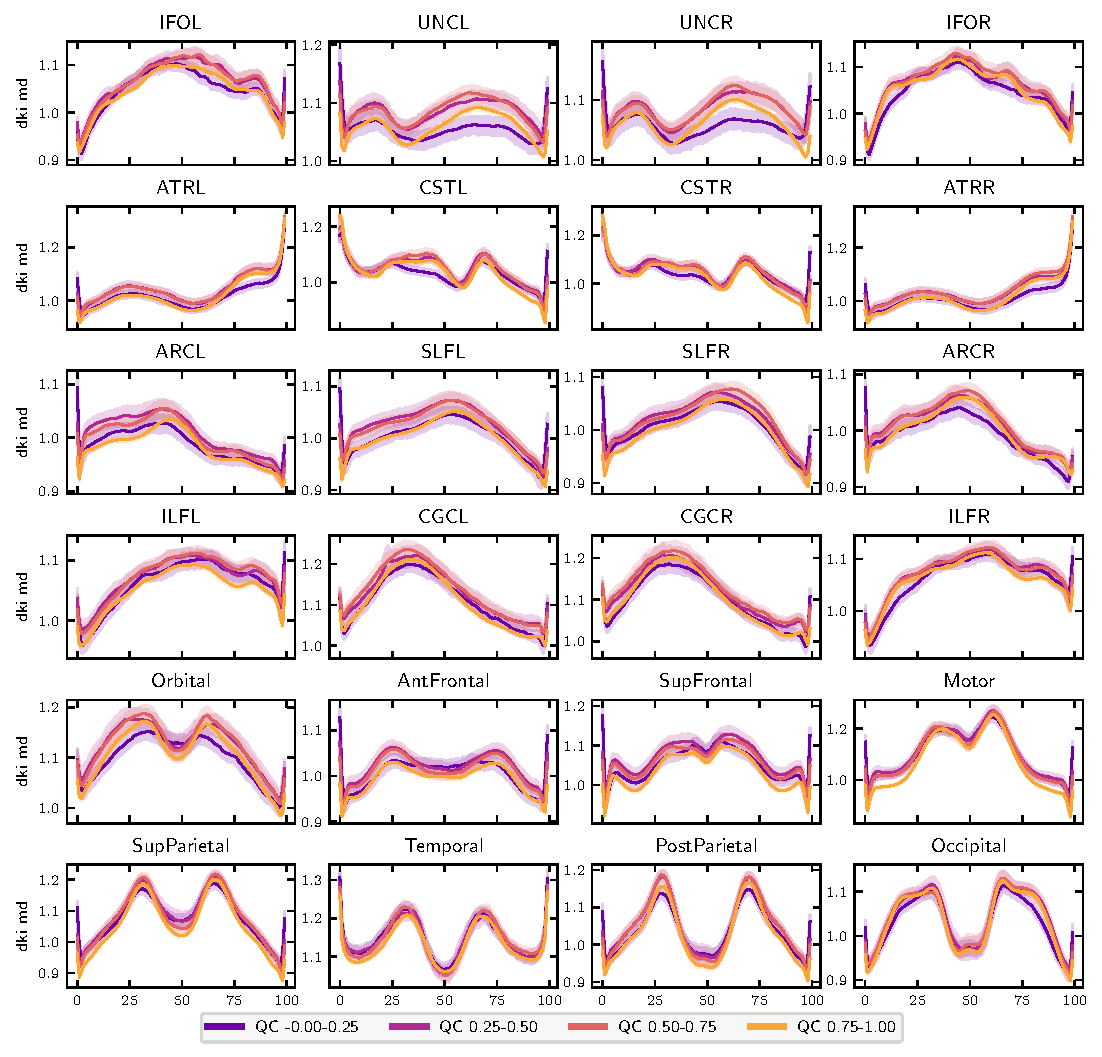
\includegraphics[width=\linewidth]{bundle-profiles/qc-bins-dki-md.pdf}
    \caption{%
        {\bf MD bundle profiles show large QC group differences}:
        MD profiles binned by QC score in twenty-four major while matter
        bundles. The left and right uncinate bundles are the most sensitive
        to QC score. Generally, QC score tends to flatten bundle profiles.
        Error bands represent bootstrapped 95\% confidence intervals. Bundle
        abbreviations for lateralized bundles contain a trailing ``L'' or ``R''
        indicating the hemisphere. Bundle abbreviations:
        inferior fronto-occipital fasciculus (IFO),
        uncinate (UNC),
        thalamic radiation (ATR),
        corticospinal (CST),
        arcuate (ARC),
        superior longitudinal fasciculus (SLF).
        inferior longitudinal fasciculus (ILF),
        cingulum cingulate (CGC),
        orbital corpus callosum (Orbital),
        anterior frontal corpus callosum (AntFrontal),
        superior frontal corpus callosum (SupFrontal),
        motor corpus callosum (Motor),
        superior parietal corpus callosum (SupParietal),
        temporal corpus callosum (Temporal),
        post-parietal corpus callosum (PostParietal), and
        occipital corpus callosum (Occipital).
    }
    \label{fig:qc-profiles:md}
\end{figure}

\arhtodo[inline]{
    The tract profile plot needs improvement. Specifically, the axes text
    takes up a lot of room so it's hard to see the plots.

    In fact, all of the plots could be improved to use the same font and fontsize
    as the text.
}

The effect of QC score on white matter bundle profiles suggests that researchers
using HBN-POD2 incorporate QC in their analyses, either by applying a QC cutoff
when selecting subjects or by explicitly added QC score to their inferential
models. Failure to do so may cause spurious associations or degrade predictive
performance. To demonstrate this, we select participant age as a representative
phenotypic benchmark \cite{cole2019brain,richie-halford2021multidimensional} and
observed the effect of varying QC cutoff on the predictive performance of an age
prediction model. Cross-validated $R^2$ scores for an age prediction model
varies depending on the QC cutoff (Figure~\ref{fig:age-prediction}). An initial large improvement was achieved by excluding the 200 participants with the lowest QC scores, followed by a gradual increase in performance. Finally, when a large number of participants is excluded, performance deteriorated again.

\begin{figure}[htbp]
    \centering
    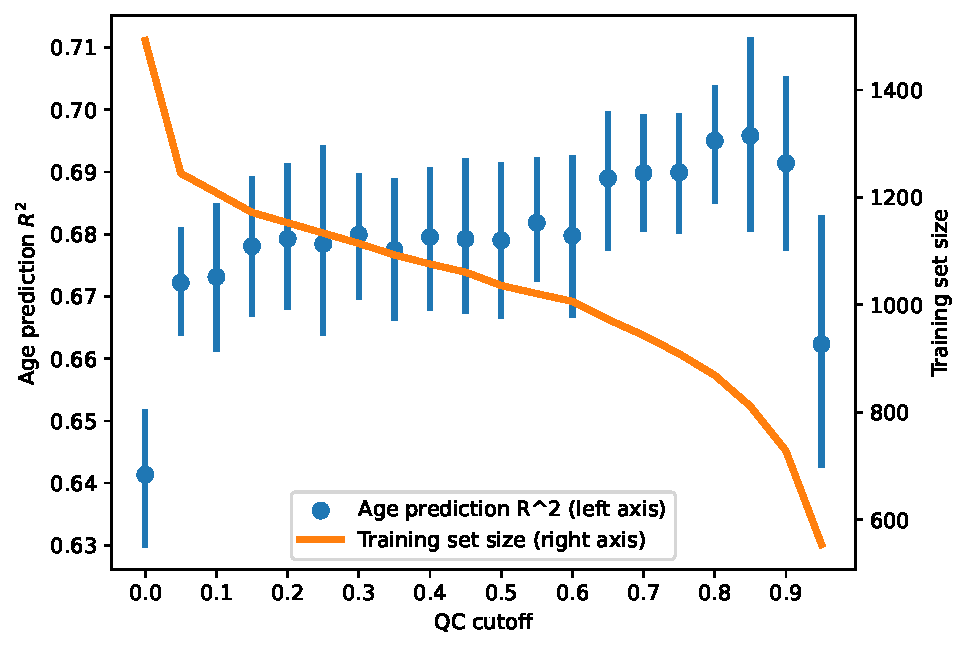
\includegraphics[width=0.5\linewidth]{age-prediction/qc_sweep.pdf}
    \caption{%
        {\bf Imposing a QC cutoff improves age prediction}:
        Cross validated $R^2$ scores (left axis, blue dots) from an age
        prediction model increase after screening subjects by QC score. We see
        the most dramatic increase in $R^2$ after imposing even the lowest
        cutoff of $0.05$. Thereafter, the $R^2$ scores trend upward until a
        cutoff of $\sim 0.95$, where the training set size (right axis, orange
        line) becomes too small to sustain model performance. The error bands
        represent a bootstrapped 95\% confidence interval.
    }
    \label{fig:age-prediction}
\end{figure}

\section*{Discussion}

We present HBN-POD2, one of the largest child and adolescent diffusion imaging
datasets with derived measures that is currently openly available. The dataset
was designed to comply with the best practices of the field. For example, it
complies with the current draft of the BIDS diffusion derivative specification
\cite{Pestilli2021}. It will grow continuously as the HBN study acquires more
data, eventually reaching its \num{10000} subject goal. Here we summarize the
contributions of this work, starting from the potential impact of the range of
resources we have created and ending with implications for processing and
quality control of other large-scale datasets.

\subsection*{Standardized preprocessing and quality control increase the impact of openly-available data}

The most immediate contribution of this work is a large analysis-ready dMRI
dataset, openly accessible to the public. In the past decade, projects such as
the Human Connectome Project (HCP) \cite{van-essen2013-oi}, UK Biobank
\cite{miller2016-mq}, ABCD \cite{jernigan2018-my}, and CamCAN
\cite{taylor2017-or,shafto2014-ld} and of course FCP-INDI (which includeds HBN)
\cite{Mennes2013-eu} have ushered a culture of data sharing in open big-data
neuroscience. The adoption and reuse of these datasets reduces or eliminates the
data collection burden on downstream researchers. Some projects, such as the HCP
\cite{glasser2013-lo}, also provide preprocessed derivatives, further reducing
researchers' burden and extending the benefits of data-sharing from data
collection to preprocessing and secondary analysis. Following the example of the
HCP, HBN-POD2 provides analysis-ready dMRI derivatives. This avoids duplication
of preprocessing effort while also ensuring a minimum standard of data quality
for HBN researchers. The data is amenable to many different analyses, including
tractometry \cite{yeatman2012-rc}, graph theoretical analysis \cite{yeh2020-nu},
and combinations with functional MRI data and other data types for the same
subjects. The availability of standardized preprocessed diffusion data will
allow researchers to create and test hypotheses on the white matter properties
underlying behavior and disease, from reading and math acquisition to childhood
adversity and mental health. As such, this dataset will accelerate discovery at
the nexus of structural connectivity and neurodevelopmental and learning
disorders.

In this kind of dataset, it is important to perform accurate and reliable QC of
the data.  HBN-POD2 provides four separate QC scores alongside its large dataset
of pediatric neuroimaging diffusion derivatives, paving the way for users of the
data to incorporate considerations of data quality into their analysis of the
processed data. Unsurprisingly, QC scores are strongly directly correlated with
age (Figure~\ref{fig:dl-qc}). This accords with the negative association
between head motion and age, which is well established both in general
\cite{power2012spurious,satterthwaite2012impact,fair2012distinct,yendiki2014spurious}
and specifically for resting-state fMRI in the HBN dataset \cite{alexander2017-yc}.

We demonstrate the impact of QC in a benchmark age prediction task
(Figure~\ref{fig:age-prediction}). In this case, the increase in model performance
from imposing a QC cutoff is intuitive: we know from
Figure~\ref{fig:qc-profiles:md} that participants with low QC scores have
reduced MD, but MD also decreases as subjects mature
\cite{yeatman2014lifespan,richie-halford2021multidimensional}. Eliminating
subjects with low QC therefore removes subjects who may look artificially older
from the analysis, improving overall performance. The most noticeable
improvement in performance comes after imposing the most modest cutoff of
$0.05$, suggesting that inferences may benefit from \emph{any} QC screening. On
the other hand, QC screening inherently introduces a tension between the desire
for high quality data and the desire for a large sample size. In this case,
after a QC cutoff of around $0.9$, the training set size is reduced such that it
degrades predictive performance. Importantly, we do not expect the sensitivity
analysis of an age prediction model to generalize to other analyses and
recommend that researchers using HBN-POD2 conduct their own.

\subsection*{Automated quality control: a tension between scalability and interpretability}

We provide four different scores in anticipation of end-user's reluctance to
trust a QC score generated through deep learning \cite{lipton2017doctor,
Zech2018-ki, Ghassemi2021-zg, salahuddin2022transparency}. The predictive
performance of the CNN-i model (Figure~\ref{fig:dl-qc:roc}) gives
us confidence that it could accurately classify unseen data, justifying its
extension to the entire HBN-POD2 dataset and to future releases. However, it
does not explain its decisions. As deep learning models have been increasingly
applied to medical image analysis, there is an evolving interest in the
interpretability of these models \cite{salahuddin2022transparency}. While an
exhaustive interpretation of deep learning QC models is beyond the scope of this
work, we provided a preliminary qualitative interpretation of the CNN-i model
(Figure~\ref{fig:ig}) that demonstrates the intuitive nature of its decisions.

Nevertheless, we recognize that some researchers may still be leery of the deep
learning generated scores. Therefore, in addition to the deep learning generated
scores, we provide
\begin{enumerate*}[%
    label=(\roman*),%
    before=\unskip{ },%
    itemjoin={{, }},%
    itemjoin*={{ and }}]
    \item the mean expert QC score for the 200 subjects in the gold standard
    dataset
    \item the scores predicted by the XGB model, which outperformed all other models
    when evaluated against the gold standard ratings, but which are only available
    for participants that have community science scores
    \item the scores predicted by the XGB-q model, which underperformed the deep
    learning generated scores, but which rely only on the automated QC metrics
    output by \emph{QSIPrep}.
\end{enumerate*}
We view the XGB-q scores, which are available for all participants, as a more interpretable fallback for users who are not
comfortable basing study exclusion decisions on a deep learning model
\cite{rudin2019stop}. The decision to use a more interpretable but slightly less
performant method of generating QC scores was also advocated by Tobe et
al.~\cite{tobe2021longitudinal}, who noted that the Euler number of T1-weighed
images in the NKI-Rockland dataset can reliably predict scores generated with
\emph{Braindr}, the community science application developed in our previous work
\cite{keshavan2019-er}.

We also note that the issue of algorithmic impact in choosing a QC method is not
exclusive to the deep learning model. We have chosen models that most reliably
reproduce the gold standard ratings, but a reliable algorithm might still
negatively influence researcher's decisions. For example, excluding participants
by QC score could spur them to exclude populations deserving of study, as when
QC score is highly correlates with age or socio-economic status. We therefore
caution researchers to examine interactions between the QC scores we provide and
their phenotype of interest.

More generally, QC in the dataset that we have produced is fundamentally
anchored to the decisions made by the expert observers. While Cohen's $\kappa$
between some pairs of experts can be as low as 0.52, IRR quantified across all
of the experts with ICC3k is excellent. Nevertheless, it is possible that
improvements to the final QC scores could be obtained through improvements to
IRR, or by designing a more extensive expert QC protocol. The tradeoff between
more extensive QC for each subject and more superifcial QC on more subjects was
not explored in this study, but could also be the target for future research.

\subsection*{Fully transparent pipelines provide an extensible baseline for future methods development}

While the primary audience of HBN-POD2 is researchers in neurodevelopment who
will use the dMRI derivatives in their studies, other researchers may use
HBN-POD2 to develop new preprocessing algorithms or quality control methods. In
this respect, HBN-POD2 follows Avesani et al.~\cite{avesani2019-ey}, who
recognized the diverse interests that different scientific communities have in
reusing neuroimaging data and coined the term \emph{data upcycling} to promote
multiple-use data sharing for purposes secondary to those of the original
project. Complementing the approach taken in Avesani et al.'s work, which
provided dMRI from a small number of subjects preprocessed with many pipelines,
HBN-POD2 contains many subjects, all processed with a single state of the art
pipeline, \emph{QSIPrep}. For researchers developing new preprocessing
algorithms, HBN-POD2 provides a large, openly available baseline to which they
can compare their results.

Similarly, neuroimaging QC methods developers will benefit from a large
benchmark dataset of expert, community science and automated QC, with which to
pilot new QC methods. Importantly, the deep learning network architecture for QC
and parameters are also provided as part of this work, allowing application of
this network to future releases of HBN data, and allowing other researchers to
build upon and improve upon this work. Indeed, in this work, we have extended
our previous work on what we now call ``hybrid QC''. This approach, which we
originally applied to the HBN T1-weighted data \cite{keshavan2019-er} (using the
\emph{Braindr} web app: \url{https://braindr.us}) was extended here in several
respects
\begin{enumerate*}[%
    label=(\roman*),%
    before=\unskip{: },%
    itemjoin={{ }},%
    itemjoin*={{ }}]
    \item The \emph{Braindr} study used a smaller dataset of approximately 700
    subjects, while we extended this approach to more than \num{2000} subjects
    here.
    \item \emph{Braindr} relied on approximately \num{80000} ratings from
    \num{261} users. Here, we received more than \num{500000} ratings from
    \num{374} community scientists. As our understanding of the role of
    community scientist contributions has evolved, we decided that we would
    include as collective co-authors community scientists who contributed more
    than \num{3000} ratings \cite{Ward-Fear2020-zq}.
    \item \emph{Braindr} used data from only a single site. Here, multi-site
    data was used. This opens up multiple possibities for deeper exploration of
    between-site quality differences, and also for harmonization of QC across
    sites.
    \item The most challenging extension of hybrid QC from \emph{Braindr} to
    this study entailed developing an approach that would encompass multi-volume
    dMRI data. On the one hand, this meant that the task performed by the expert
    observers was more challenging, because it required examination of the full
    dMRI time-series for every scan. On the other hand, it also meant that the
    4D data had to be summarized into 2D data to be displayed in the \emph{Fibr}
    web application. This was achieved by summarizing the entire time-series as
    a DEC-FA + $b=0$ image and presenting community scientists with animated
    sections of these images that showed how the data extended over several
    horizontal slices. In addition, the extension to 4D data required developing
    new deep learning architectures for analysis of 4D images, including
    upstream contributions to \emph{Nobrainer}, a community-developed software
    library for deep learning in neuroimaging data \cite{nobrainer}.
\end{enumerate*}
These extensions demonstrate that the hybrid QC approach generalizes very well
to a variety of different circumstances. Future applications of this approach
could generalize to functional MRI data, as well as other large datasets from
other kinds of measurements and other research domains.

\arhtodo[inline]{%
    Add XGB-q QC scores to the \texttt{participants.tsv} on FCP-INDI in the
    ``xgb\_qsiprep\_qc\_score'' column.
}

\arhtodo[inline]{%
    Add some text about the benefit of generalizing the hybrid approach to
    multisite and multi-modality data. Also need to discuss comparison with
    previous T1-weighted work. One thing to discuss there is that expert
    inter-rater reliability was *a lot* higher for T1-weighted. This is
    potentially a problem, but also highlights how important it is to have an
    automated, ``objective'' approach.
}

\subsection*{Future work and open problems}

The HBN study plans to acquire imaging data for \num{10000} participants,
necessitating future data releases. Future releases of HBN will require future
releases of HBN-POD2, and a plan for these future releases is essential. This is
a general issue affecting multi-year neuroimaging projects for which derivative
data is being released before study completion. The use of \emph{QSIPrep},
\emph{cloudknot} and the containerization of the QC score assignment process
facilitate running the exact pipeline described in this paper on newly released
subjects. However, this approach is somewhat unsatisfactory because it fails to
anticipate improvements in preprocessing methodology. That is, what should we do
when \emph{QSIPrep} is inevitably updated between HBN releases? Enforce
standardization by using an outdated pipeline or use state-of-the-art
preprocessing at the expense of standardized processing between releases?
Because the use of \emph{cloudknot} and AWS Spot Instances renders preprocessing
fast and relatively inexpensive, we propose a third way: if improvements to the
preprocessing pipeline are available with a new HBN release, we plan to execute
the improved pipeline on the entire HBN dataset, while preserving the previous
baseline release in an archived BIDS derivative dataset.

Undertaking the processing and QC effort to generate HBN-POD2 required
construction and deployment of substantial informatics infrastructure, including
tools for cloud computing, web applications for expert annotation and for
community science rating and analysis software. All of these tools are provided
openly, so that this approach can be generalized even more widely in other
projects and in other scientific fields.

\rokemtodo[inline]{%
    After we run the site generalization experiments, speculate about
    generalization to other datasets. We should point out ABCD in particular
    since the CUNY and CBIC sites are supposed to be harmonized with ABCD. This
    discussion will hinge on the results of the remaining multi-site
    generalization experiments.
}

\section*{Methods}

To facilitate replicability, Jupyter notebooks \cite{kluyver2016jupyter} and
Dockerfiles \cite{merkel2014docker} necessary to reproduce the methods described
herein are provided in the HBN-POD2 GitHub repository at
\url{https://github.com/richford/hbn-pod2-qc}. The specific version of the
repository used in this study is also available at
\url{https://doi.org/our.awesome.doi}. The \texttt{make} or \texttt{make help}
commands will list the available commands and \texttt{make build} will build the
requisite Docker images to analyze HBN-POD2 QC data. In order to separate data
from analysis code \cite{Wilson2017-rj}, we provide intermediate data necessary
to analyze the QC results in an OSF \cite{Foster-MSLS2017-rl} project
\cite{hbn-pod2-osf}, which can be downloaded using the \texttt{make data}
command in the root of the HBN-POD2 GitHub repository. Most of the code in this
repository uses Pandas \cite{mckinney-proc-scipy-2010,reback2020pandas}, Numpy
\cite{harris2020array}, Matplotlib \cite{hunter2007matplotlib}, and Seaborn
\cite{waskom2021seaborn}.
\arhtodo[inline]{Zenodo the Github repo and add a citation here.}

Inputs for this study consisted of MRI data from the Healthy Brain Network
pediatric mental health study \cite{alexander2017-yc}, containing dMRI data from
\num{2747} subjects with ages 5-21. These data were measured using a
\qty{1.5}{\tesla} Siemens mobile scanner on Staten Island (SI) and three fixed
\qty{3}{\tesla} Siemens MRI scanners at sites in the New York area: Rutgers
University Brain Imaging Center (RUBIC), the CitiGroup Cornell Brain Imaging
Center (CBIC), and the City University of New York Advanced Science Research
Center (CUNY). Informed consent was obtained from each participant aged 18 or
older. For participants younger than 18, written consent was obtained from their
legal guardians and written assent was obtained from the participant. Voxel
resolution was \qty{1.8}{\mm} $\times$ \qty{1.8}{\mm} $\times$ \qty{1.8}{\mm} with \num{64} non-colinear
directions measured for each of $b=1000$ \unit{\second \per \mm^{2}} and
$b=2000$ \unit{\second \per \mm^{2}}.

\subsection*{BIDS curation}

We curated the imaging metadata for \num{2615} of the \num{2747} currently
available HBN subjects. Using dcm2bids and custom scripts, we conformed the data
to the Brain Imaging Data Structure (BIDS; \cite{gorgolewski2016-lh})
specification. The BIDS-curated dataset is available on FCP-INDI and can be
accessed via AWS S3 at \url{s3://fcp-indi/data/Projects/HBN/BIDS_curated/}.

\mctodo[inline]{Add more BIDS curation information}

\subsection*{Preprocessing}

We performed dMRI preprocessing on \num{2136} subjects, using \emph{QSIPrep}
\cite{cieslak2021-iq} 0.12.1, which is based on \emph{Nipype} 1.5.1
\cite{nipype1,nipype2}, RRID:SCR\_002502. \emph{QSIPrep} a robust and scalable
pipeline to group, distortion correct, motion correct, denoise, coregister and
resample MRI scans. In total, \num{417} subjects failed this preprocessing
step, largely due to missing dMRI files. In keeping with the BIDS specification,
the preprocessed dataset is available as a derivative dataset within the
BIDS-curated dataset and can be access on AWS S3 at
\url{s3://fcp-indi/data/Projects/HBN/BIDS_curated/derivatives/qsiprep/}.
\emph{QSIPrep} fosters reproducibility by automatically generating thorough
methods boilerplate for later use in scientific publications, which we use for
the remainder of this subsection to document each preprocessing step.

\begin{itemize}

\item {\it Anatomical data preprocessing}
The T1-weighted (T1w) image was corrected for intensity non-uniformity (INU)
using \texttt{N4BiasFieldCorrection} \cite{n4} (ANTs 2.3.1), and used as
T1w-reference throughout the workflow. The T1w-reference was then skull-stripped
using \texttt{antsBrainExtraction.sh} (ANTs 2.3.1), using OASIS as target
template. Spatial normalization to the ICBM 152 Nonlinear Asymmetrical template
version 2009c \cite{mni}, RRID:SCR\_008796 was performed through nonlinear
registration with \texttt{antsRegistration} \cite{ants}, ANTs 2.3.1,
RRID:SCR\_004757, using brain-extracted versions of both T1w volume and
template. Brain tissue segmentation of cerebrospinal fluid (CSF), white-matter
(WM) and gray-matter (GM) was performed on the brain-extracted T1w using
\texttt{FAST} \cite{fsl-fast}, FSL 6.0.3:b862cdd5, RRID:SCR\_002823.

\item {\it Diffusion data preprocessing}

Any images with a $b$-value less than \qty{100}{\second \per \mm^{2}} were treated
as a $b=0$ image. MP-PCA denoising as implemented in MRtrix3's
\texttt{dwidenoise}\cite{dwidenoise1} was applied with a 5-voxel window. After
MP-PCA, B1 field inhomogeneity was corrected using \texttt{dwibiascorrect} from
MRtrix3 with the N4 algorithm \cite{n4}. After B1 bias correction, the mean
intensity of the DWI series was adjusted so all the mean intensity of the $b=0$
images matched across eachseparate DWI scanning sequence.

FSL (version 6.0.3:b862cdd5)'s eddy was used for head motion correction
and Eddy current correction \cite{anderssoneddy}. Eddy was configured
with a \(q\)-space smoothing factor of 10, a total of 5 iterations, and
\num{1000} voxels used to estimate hyperparameters. A linear first level model
and a linear second level model were used to characterize Eddy
current-related spatial distortion. \(q\)-space coordinates were
forcefully assigned to shells. Field offset was attempted to be
separated from subject movement. Shells were aligned post-eddy. Eddy's
outlier replacement was run \cite{eddyrepol}. Data were grouped by
slice, only including values from slices determined to contain at least
\num{250} intracerebral voxels. Groups deviating by more than four standard
deviations from the prediction had their data replaced with imputed
values. Data was collected with reversed phase-encode blips, resulting
in pairs of images with distortions going in opposite directions. Here,
$b=0$ reference images with reversed phase encoding directions were used
along with an equal number of $b=0$ images extracted from the DWI scans.
From these pairs the susceptibility-induced off-resonance field was
estimated using a method similar to that described in \cite{topup}. The
fieldmaps were ultimately incorporated into the Eddy current and head
motion correction interpolation. Final interpolation was performed using
the \texttt{jac} method.

Several confounding time-series were calculated based on the
\emph{preprocessed DWI}: framewise displacement (FD) using the implementation
in \emph{Nipype} following the definitions by \cite{power-fd-dvars}. The DWI
time-series were resampled to ACPC, generating a \emph{preprocessed DWI run
in ACPC space}.

\end{itemize}

Many internal operations of \emph{QSIPrep} use \emph{Nilearn} 0.6.2
\cite{nilearn}, RRID:SCR\_001362 and \emph{DIPY} \cite{dipy}. For more details
of the pipeline, see
\href{https://qsiprep.readthedocs.io/en/latest/workflows.html}{the section
corresponding to workflows in \emph{QSIPrep}'s documentation}.

\subsection*{Cloud-based distributed preprocessing}

The containerization of \emph{QSIPrep} provided a consistent preprocessing
pipeline for each subject but the number of subjects made serial processing of
each particpant prohibitive on a single machine. We used \emph{cloudknot}, a
previously developed cloud-computing library \cite{cloudknot} to
parallelize the preprocessing over individual subjects on spot instances in the
Amazon Web Services Batch service. \emph{Cloudknot} takes as input a
user-defined Python function and creates the necessary AWS infrastructure to map
that function onto a range of inputs, in this case, the subject IDs. The Python
preprocessing function was a thin wrapper around \emph{QSIPrep}'s command line
interface and is provided in a jupyter notebook in the HBN-POD2 GitHub
repository in the ``notebooks'' directory. Using \emph{cloudknot} and AWS Batch
Spot Instances, the preprocessing cost less than \textdollar1.00 per subject.

\subsection*{Expert quality control}

The expert QC ``gold standard'' subset was created by randomly selecting 200
subjects from the preprocessed dataset, sampled such that the proportional site
distribution in the gold standard subset matched that of the preprocessed
dataset.

We created a web application for expert quality control of preprocessed dMRI,
called \emph{dmriprep-viewer} \cite{richie-halford2021-viewer}. The viewer
ingests \emph{QSIPrep} outputs and generates a browser-based interface for
expert QC. It provides a study overview page displaying the distributions of
\emph{QSIPrep}'s automated QC metrics (described at
\url{https://qsiprep.readthedocs.io/en/latest/preprocessing.html#quality-control-data}).
Each datum on the study overview page is interactively linked to a subject-level
QC page that provides an interactive version of \emph{QSIPrep}'s visual reports
(described at
\url{https://qsiprep.readthedocs.io/en/latest/preprocessing.html#visual-reports}).
The viewer allows users to assign a rating of $-2$ (definitely fail), $-1$
(probably fail), $0$ (not sure), $1$ (probably pass), or $2$ (definitely pass) to a
subject. To standardize rater expectations before rating, expert raters watched
a tutorial video (which is available in the OSF project). They then rated each
subject and saved their scores and sent them to the lead author for compilation.

\comment[inline]{%
    The new viewer will be called NIRV, the neuroimaging report viewer and we'll
    write another paper about that. So lots of details about the implementation
    are witheld from this paper.
}

To compute the pairwise Cohen's $\kappa$ scores in Figure~\ref{fig:expert-qc:irr}, we
used the \emph{scikit-learn} \cite{scikit-learn} \texttt{cohen\_kappa\_score}
function with quadratic weights. To compute intraclass correlation, we used the
\emph{pingouin} statistical package \cite{vallat2018pingouin}
\texttt{intraclass\_corr} function. The expert rating analysis can be replicated
using the \texttt{make expert-qc} command in the HBN-POD2 GitHub repository.
The mean expert ratings, scaled to the range $[0, 1]$ are available in the
``expert\_qc\_score'' column of the \texttt{participants.tsv} file on FCP-INDI.

\subsection*{Community scientist quality control}

The community science web application is based on the SwipesForScience framework
\url{https://swipesforscience.org/}, which generates a web application for
community science given an open repository of images to be labelled and a
configuration file. The source code for the \emph{Fibr} web application is
available at \url{https://github.com/richford/fibr}. After a brief tutorial,
community scientists provided binary pass/fail ratings based on the DEC-FA from
a fit of a DTI model to each subject's preprocessed dMRI data. These images were
generated using a \emph{DIPY} \cite{dipy} \texttt{TensorModel} in a
\emph{cloudknot}-enabled Jupyter notebook that is available in the ``notebooks''
directory of the \emph{Fibr} GitHub repository. \emph{Fibr} saves each community
rating to its Google Firebase backend, the contents of which have been archived
to the HBN-POD2 OSF project.

The \emph{Fibr} ratings were then combined with automated \emph{QSIPrep} QC
metrics to train the gradient boosted trees models XGB, XGB-f, and XGB-q. These
models were implemented as binary classifiers using the XGBoost library
\cite{xgboost}. The targets for these classifiers were the mean expert ratings
in the gold standard dataset, rescaled to the range $[0, 1]$ and binarized with
a threshold of $0.5$. Using repeated
stratified K-fold cross-validation, with three splits and two repeats, we
evaluated the models' performance in predicting the gold standard ratings. In
each fold, the best model hyperparameters were chosen using the scikit-optimize
\cite{scikit-optimize} \texttt{BayesSearchCV} class. Saved model checkpoints for
each cross-validation split are available in the HBN-POD2 OSF project. Since
each split resulted in a different XGB model and we required a single QC score
to train the deep learning model, we combined the models from each
cross-validation split using a voting classifier, computing a weighted averaged
of the predicted probability of passing from each model, weighted by its
out-of-sample ROC AUC. This was implemented using scikit-learn's
\texttt{VotingClassifier} class. Treating the voting classifier as another
``expert'' rater, we reassessed the pairwise Cohen's $\kappa$ and ICC scores as
in the expert QC subsection. The community ratings analysis can be replicated
using the \texttt{make community-qc} command in the HBN-POD2 GitHub repository.
The XGB model's positive class probabilities are available in the
``xgb\_qc\_score'' column of the \texttt{participants.tsv} file on FCP-INDI, while
the XGB-q model's positive class probabilities are available in the
``xgb\_qsiprep\_qc\_score'' column.

\subsection*{Deep learning to predict quality control}

\begin{figure}[tbp]
    \begin{subfigure}[t]{0.6\textwidth}
    \centering
    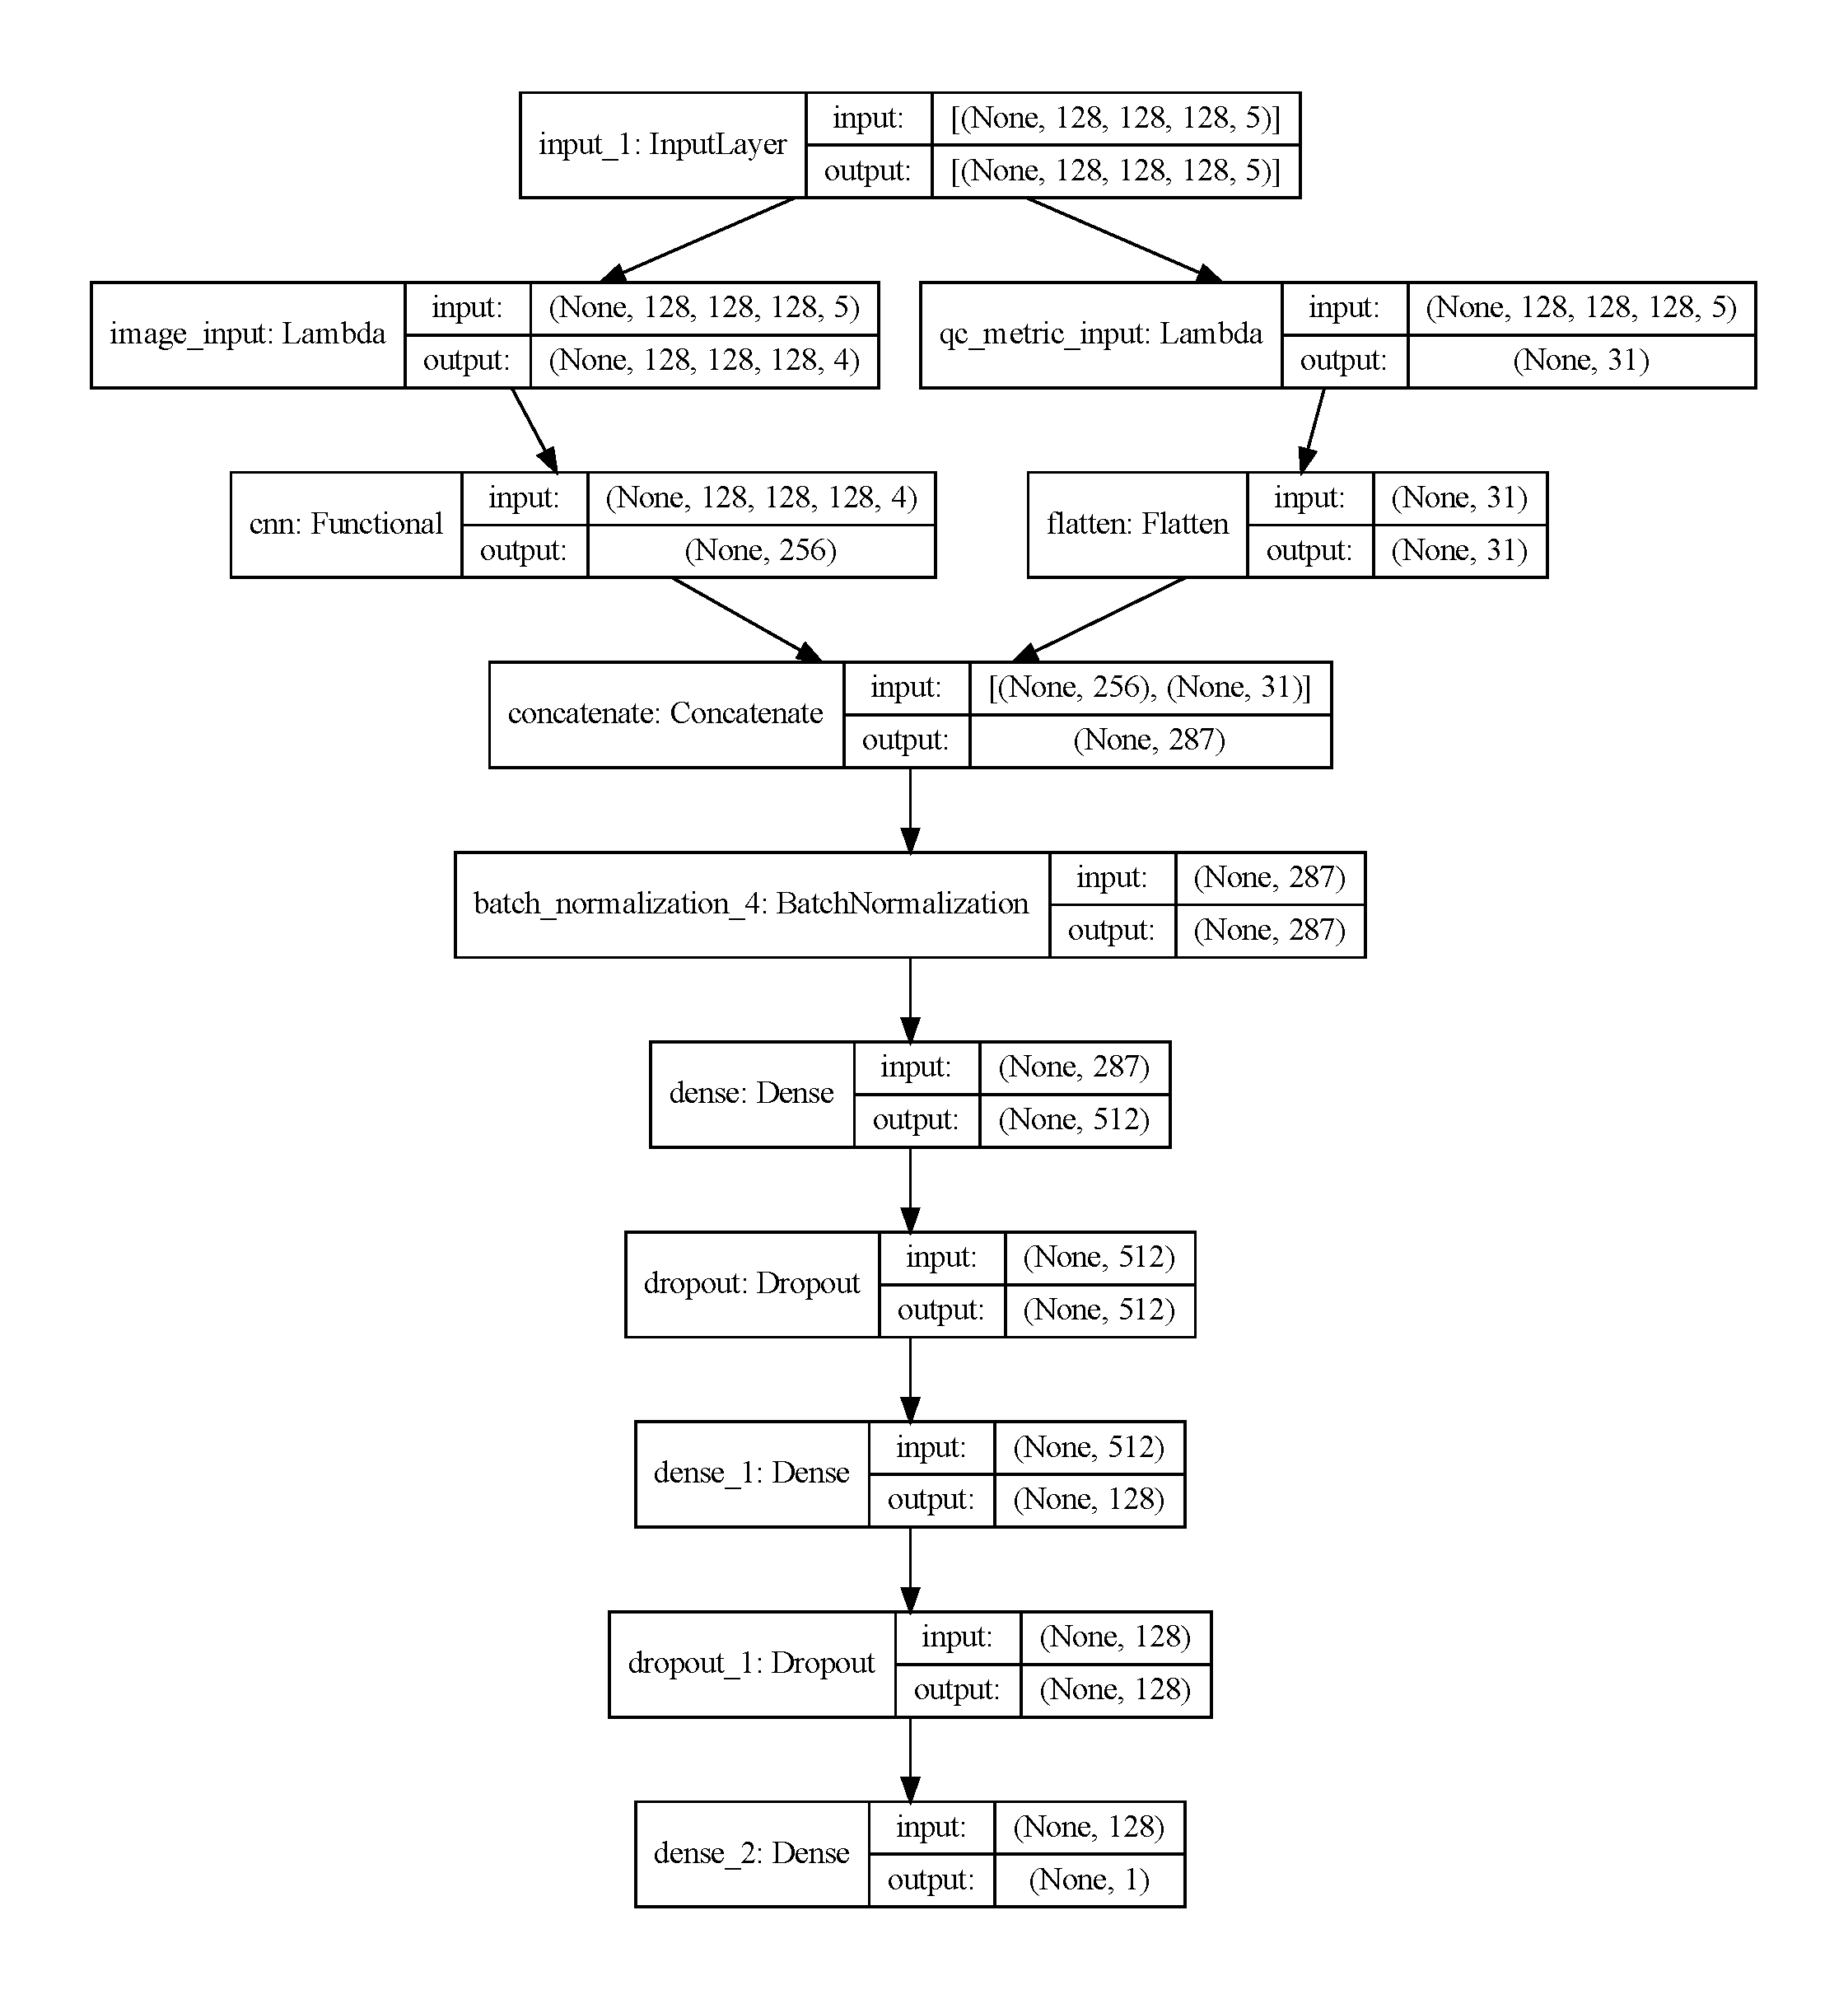
\includegraphics[width=\linewidth]{deep-learning-qc/model.pdf}
    \caption{Slicing and combining the input channels}
    \label{fig:dl-architecture:complete}
    \end{subfigure}
    \begin{subfigure}[t]{0.4\textwidth}
    \centering
    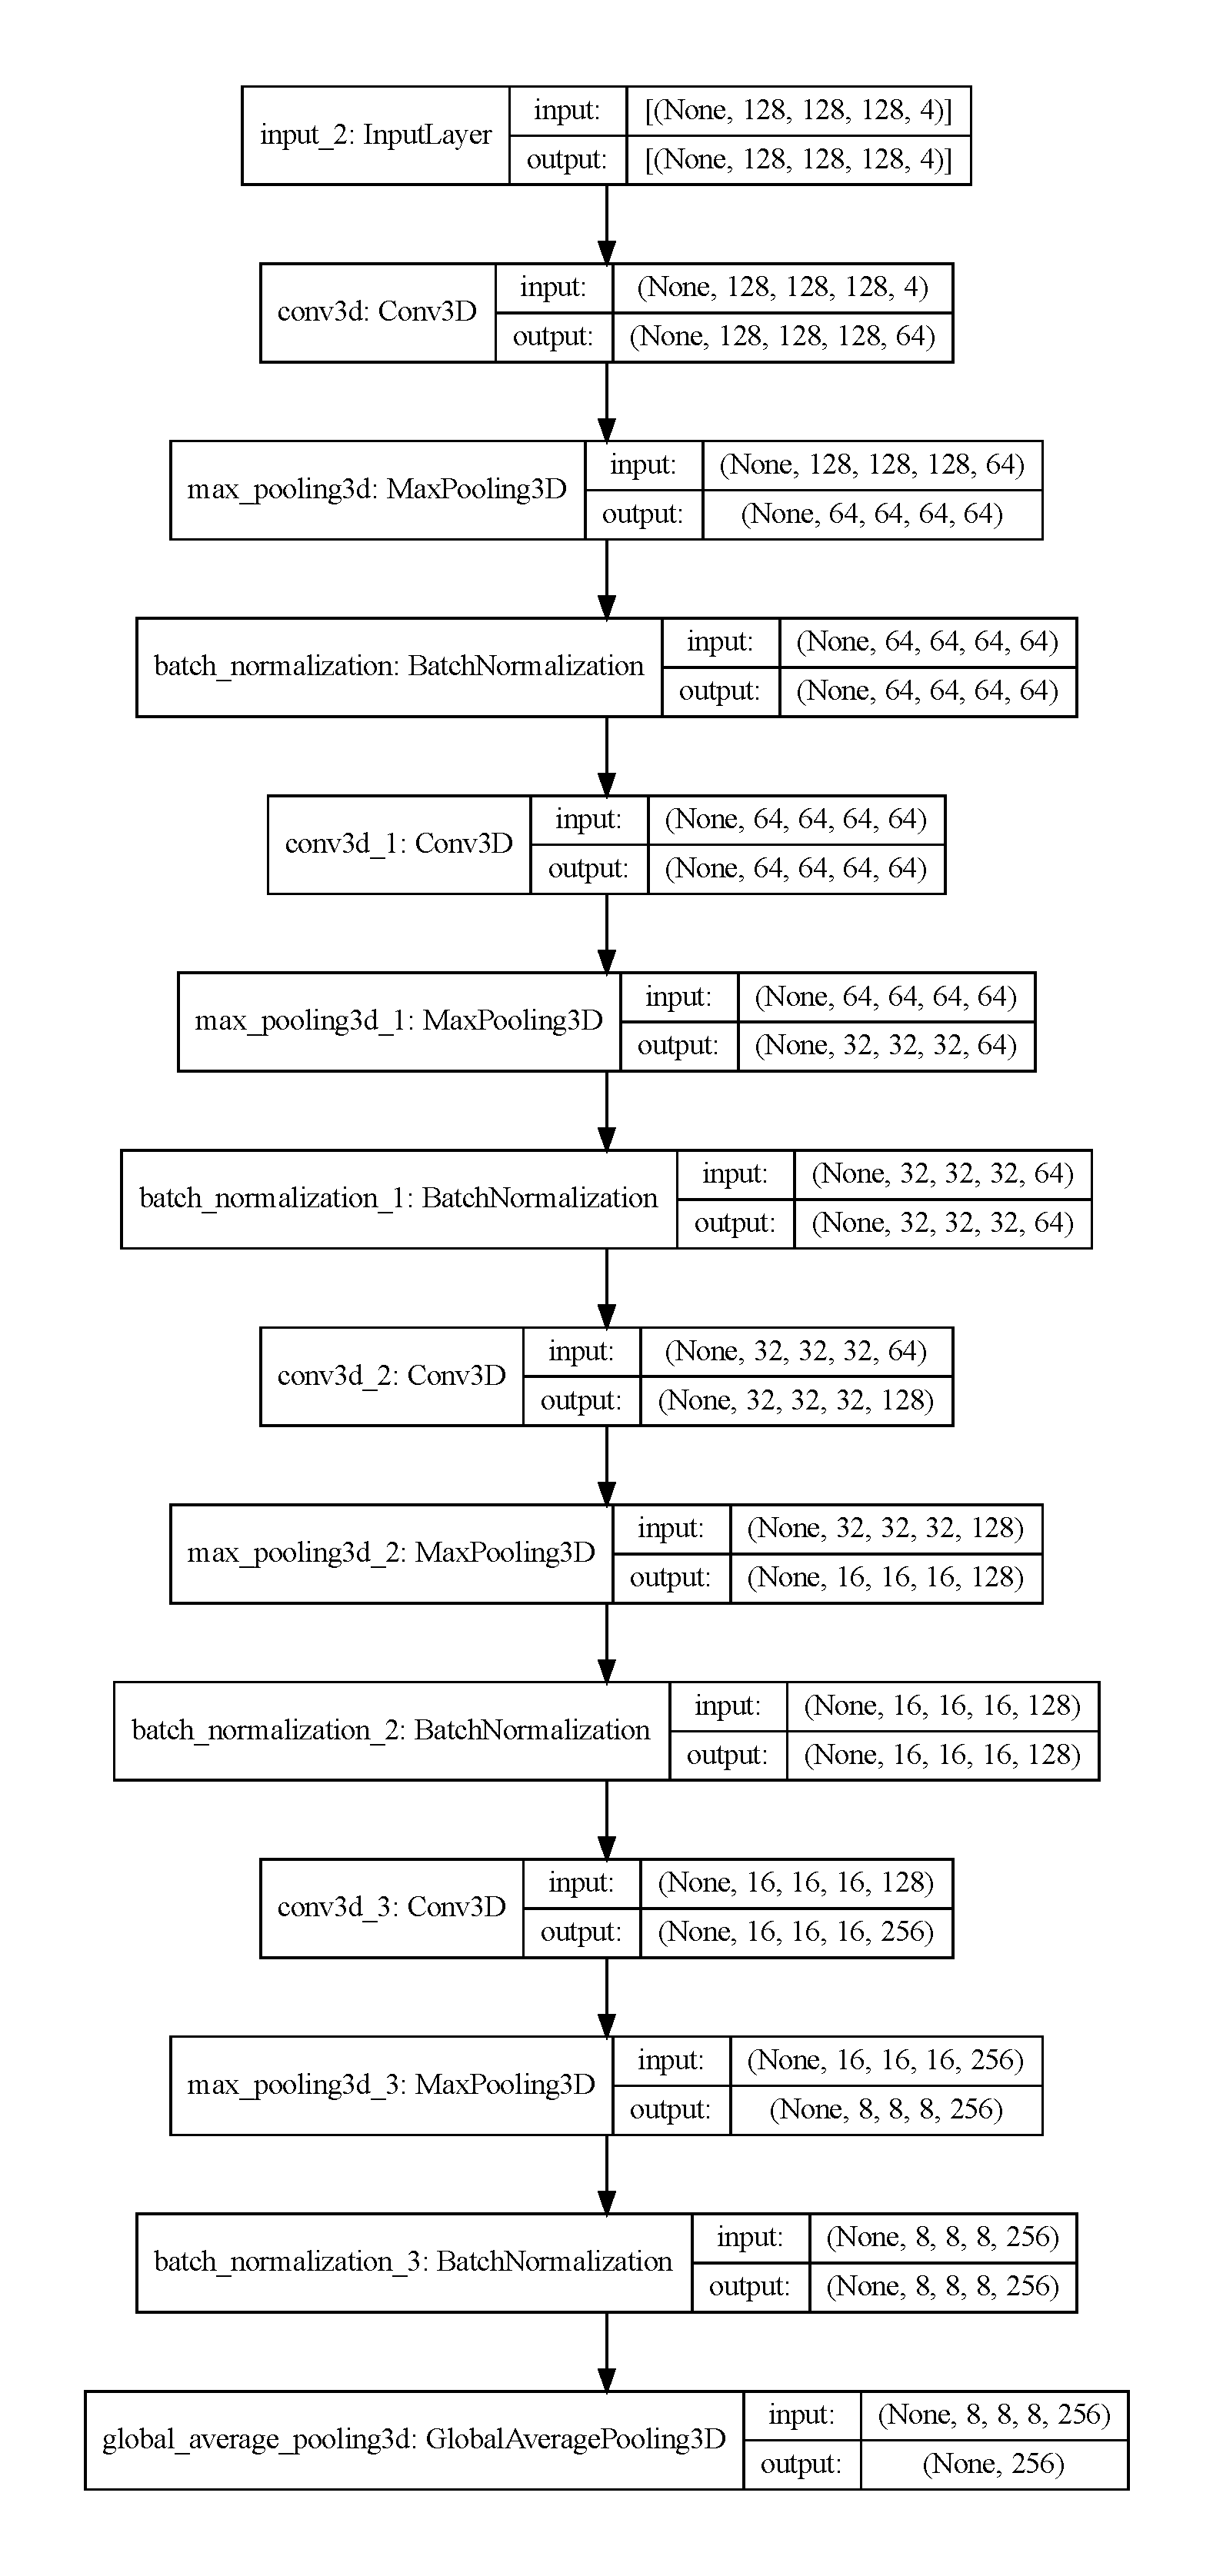
\includegraphics[width=\linewidth]{deep-learning-qc/image_model.pdf}
    \caption{CNN architecture}
    \label{fig:dl-architecture:cnn}
    \end{subfigure}
    \caption{%
        {\bf Deep learning model architecture}:
        \textbf{(a)} The CNN-i+q model accepts multichannel input that combined
        four imaging channels with a fifth channel containing 31 \emph{QSIPrep}
        automated QC metrics. The imaging channels are separated from the QC
        channel using \texttt{Lambda} layers. The imaging channels are passed
        through a CNN \textbf(b), the output of which is concatenated with the
        QC metrics, batch normalized and passed through two fully-connected (FC)
        layers, with rectified linear unit (ReLu) activation functions and with
        512 and 128 units respectively. Each FC layer is followed by a dropout
        layer which drops 40\% of the input units. The final layer contains a
        single unit with a sigmoid activation function and outputs the
        probability of passing QC.
        %
        \textbf{(b)} The CNN portion of the model passes the imaging input
        through four convolutional blocks. Each block consists of a 3D
        convolutional layer with a kernel size of 3 and a ReLu activation, a 3D
        max pooling layer with a pool size of 2, and a batch normalization layer
        with Tensorflow's default parameters. The number of filters in the
        convolutional layers in each block are 64, 64, 128, and 256 respecively.
        The output of the final block is passed through a 3D global average
        pooling layer with Tensorflow's default parameters.}
    \label{fig:dl-architecture}
\end{figure}

The binarized voting classifier's predictions were then used as targets to train a deep
learning binary classifier to predict QC scores based on each subject's preprocessed
dMRI data. We trained two different model architectures
\begin{enumerate*}[%
    label=(\roman*),%
    before=\unskip{: },%
    itemjoin={{, }},%
    itemjoin*={{ and }}]
    \item CNN-i, which took only preprocessed dMRI images as input
    \item CNN-i+q, whose input also included \emph{QSIPrep}'s automated QC metrics.
\end{enumerate*}
Both models were implemented in Tensorflow 2 \cite{tensorflow} using the Keras
module \cite{keras}. The image processing part of the model architecture was
identical for both models: a modification of an existing 3D CNN
\cite{zunair2020-bs} previously applied to the assess tuberculosis severity
\cite{dicente2019clef}. It accepts a 3D volume as input with four channels
\begin{enumerate*}[%
    label=(\roman*),%
    before=\unskip{: },%
    itemjoin={{, }},%
    itemjoin*={{ and }}]
    \item the $b=0$ reference volume
    \item DEC-FA in the $x$-direction
    \item DEC-FA in the $y$-direction
    \item DEC-FA in the $z$-direction.
\end{enumerate*}
The \emph{QSIPrep}'s automated QC metrics were included as an additional fifth
channel. The CNN-i+q model architecture is summarized in
Figure~\ref{fig:dl-architecture}. Upon input, the CNN-i+q model extracts the
imaging channels and passes them through the CNN architecture. The remaining QC
metric channel is flattened and passed ``around'' the CNN architecture and
concatenated with the output of the convolutional layers. This concatenated
output is then passed through a fully-connected layer to produce a single
output, the probability of passing QC. This architecture has \num{1438783} trainable
parameters.

We used \emph{DIPY} \cite{dipy} and \emph{cloudknot} \cite{cloudknot} to
generate these multichannel volumes for each subject and save them as NIfTI-1
files \cite{nifti}. These NIfTI files were then converted to the Tensorflow
TFRecord format using the \emph{Nobrainer} deep learning framework
\cite{nobrainer}.
\arhtodo[inline]{%
    Before submission, ask the \emph{Nobrainer} folks to cut a new release that
    contains Adam's contributions so that we are referencing the correct
    version. This cites a previous version that will not accept multichannel
    volumes.
}
The Jupyter notebooks used to create these NIfTI and TFRecord files are
available in the ``notebooks'' directory of the \emph{Fibr} GitHub
repository.

We trained each model using the Google Cloud AI Platform Training service and
the HBN-POD2 GitHub repository contains Docker services to launch training (with
\texttt{make dl-train}) and prediction (with \texttt{make dl-predict}) jobs on
Google Cloud, if the user has provided the appropriate credentials in an
environment file and placed the TFRecord files on Google Cloud Storage. To
estimate the variability in model training, we trained ten separate models using
different training and validation splits of the data. The gold standard dataset
was not included in any of these splits and was reserved for reporting final
model performance. Models were optimized for binary crossentropy loss using the
Adam optimizer \cite{kingma2017adam} with an initial learning rate of 0.0001. We
reduced the learning rate by a factor of 0.5 when the validation loss plateaued
for more than two epochs. We also stopped training when the validation loss
failed to improve by more than 0.001 for twenty consecutive epochs. These two
adjustments were made using the \texttt{ReduceLROnPlateau} and
\texttt{EarlyStopping} callbacks in Tensorflow 2 \cite{tensorflow} respectively.
The training and validation loss curves for both the CNN-i and CNN-i+q models
are depicted in Figure~\ref{fig:dl-loss}. While the CNN-i+q model achieved
better validation loss, it did not outperform the CNN-i model on the held out
gold standard dataset. The CNN-i+q model's positive class probabilities are
available in the ``dl\_qc\_score'' column of the \texttt{participants.tsv} file on
FCP-INDI.

\begin{figure}[tbp]
    \begin{subfigure}[t]{0.5\textwidth}
    \centering
    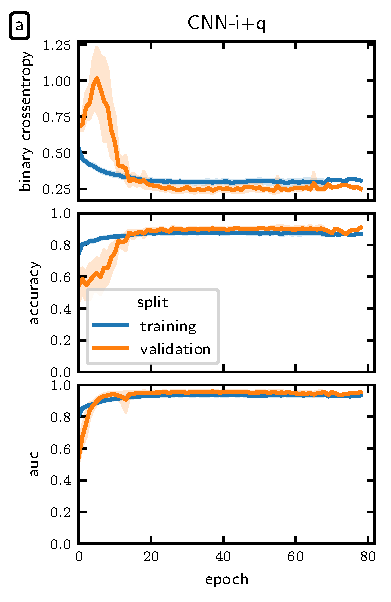
\includegraphics[width=0.9\linewidth]{deep-learning-qc/dl_learning_curve_with_qc.pdf}
    \caption{CNN-i+q}
    \label{fig:dl-loss:both}
    \end{subfigure}
    \begin{subfigure}[t]{0.5\textwidth}
    \centering
    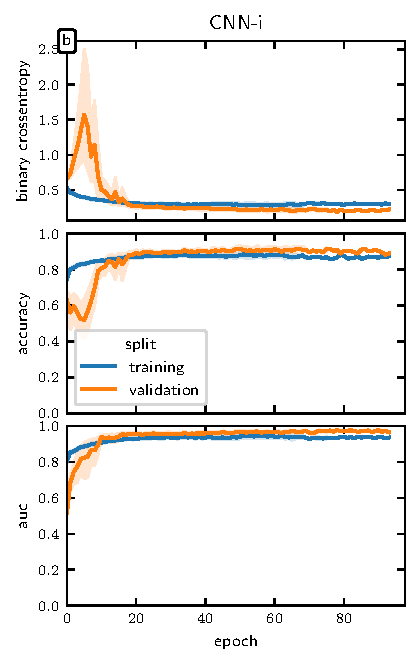
\includegraphics[width=0.9\linewidth]{deep-learning-qc/dl_learning_curve_without_qc.pdf}
    \caption{CNN-i}
    \label{fig:dl-loss:imaging}
    \end{subfigure}
    \caption{%
        {\bf Deep learning model loss curves}:
        The binary cross-entropy loss (top), accuracy (middle), and ROC AUC
        (bottom) for the CNN-i model (left) and the CNN-i+q model (right). Model
        performance typically plateaued after twenty epochs but was allowed
        continue until meeting the early stopping criterion.
        The error bands represent a bootstrapped 95\% confidence interval.
    }
    \label{fig:dl-loss}
\end{figure}

To generate the attribution maps, we followed Tensorflow's integrated gradients
tutorial \cite{integrated-gradients-tutorial} with a black baseline image and
128 steps in the Riemann sum approximation of the integral (i.e.
\texttt{m\_steps = 128}). In the HBN-POD2 GitHub repository, we provide a Docker
service to compute integrated gradient attribution maps on Google Cloud, which
can be invoked using the \texttt{make dl-integrated-gradients} command.

\subsection*{QC bundle profiles}

To generate bundle profiles, reconstruction was performed using the
\emph{QSIprep} 0.12.1 preconfigured reconstruction workflow
\texttt{mrtrix\_multishell\_msmt}, modified to generate two million streamlines
rather than the default ten million. Multi-tissue fiber response functions were
estimated using the dhollander algorithm. FODs were estimated via constrained
spherical deconvolution (CSD, \cite{originalcsd, tournier2008csd}) using an
unsupervised multi-tissue method \cite{dhollander2019response,
dhollander2016unsupervised}. Reconstruction was done using MRtrix3
\cite{mrtrix3}. FODs were intensity-normalized using mtnormalize
\cite{mtnormalize}.

These tractograms were then used as input to the Python Automated Fiber
Quantification toolbox (pyAFQ) \cite{kruper2021evaluating}. Twenty-four major
tracts, which are enumerated in Figure~\ref{fig:qc-profiles:md}, were identified using
multiple criteria: streamlines are selected as candidates for inclusion in a
bundle of streamlines that represents a tract if they pass through known
inclusion ROIs and do not pass through exclusion ROIs \cite{Wakana2007-nw}. In
addition, a probabilistic atlas is used to exclude streamlines which are
unlikely to be part of a tract and to adjudicate in cases where a streamline
could belong to more than one tract \cite{Hua2008-di}. Each streamline is
resampled to 100 nodes and the robust mean at each location is calculated by
estimating the 3D covariance of the location of each node and excluding
streamlines that are more than 5 standard deviations from the mean location in
any node. Finally, a bundle profile of tissue properties in each bundle was
created by interpolating the value of MRI maps of these tissue properties to the
location of the nodes of the resampled streamlines designated to each bundle. In
each of 100 nodes, the values are summed across streamlines, weighting the
contribution of each streamline by the inverse of the mahalanobis distance of
the node from the average of that node across streamlines. This means that
streamlines that are more representative of the tract contribute more to the
bundle profile, relative to streamlines that are on the edge of the tract.

These processes create bundle profiles, in which diffusion measures are
quantified and averaged along twenty-four major fiber tracts. We retain only the
mean diffusivity (MD) and the fractional anisotropy (FA) from a diffusion
kurtosis imagin (DKI) model \cite{jensen2005-ta}, and impute missing bundles
using median imputation as implemented by \emph{scikit-learn}'s
\texttt{SimpleImputer} class. Because the HBN-POD2 bundle
profiles exhibit strong site effects \cite{richie-halford2021multidimensional},
we used the ComBat harmonization method to robustly adjust for site effects in
the tract profiles. Initially designed to correct for site effects in gene
expression studies \cite{Johnson2007-kl}, ComBat employs a parametric empirical
Bayes approach to adjust for batch effects and has since been applied to
multi-site cortical thickness measurements \cite{fortin2018-hk}, multi-site DTI
studies \cite{fortin2017-be}, and functional MRI data in the Adolescent Brain
Cognitive Development Study (ABCD) \cite{nielson2018detecting}. We rely on the
\emph{neurocombat\_sklearn} library \cite{neurocombat-sklearn}, to apply ComBat in
before plotting bundle profiles in Figure~\ref{fig:qc-profiles:md} using
plotting functions from the AFQ-Insight package
\cite{richie-halford2019insight}. The bundle profile analysis can be replicated
using the \texttt{make bundle-profiles} command in the HBN-POD2 GitHub
repository.

\subsection*{Brain age prediction}

We evaluated the effect of varying the QC cutoff on model performance by
observing cross-validated $R^2$ values of gradient boosted trees models
implemented using XGBoost. The input feature space for each model consisted of
\num{4800} features per subject, comprising 100 nodes for each of MD and FA in
the twenty-four major tracts. We imputed missing bundles and harmonized the
different scanning sites as above. The XGBoost models' hyperparameters were
hand-tuned to values that have been performant in the authors' previous
experience. We log-transformed each participant's age before prediction using
\emph{scikit-learn}'s \texttt{TransformedTargetRegressor} class. For each value
of the QC cutoff between 0 and 0.95, in steps of 0.05, we computed the
cross-validated $R^2$ values using \emph{scikit-learn}'s
\texttt{cross\_val\_score} function with repeated K-fold cross-validation using
five folds and five repeats. Note that the practice of whole dataset imputation
before cross-validation permits the possibility of dataset leakage between train
and test splits. Similarly, sequential hand-tuning of hyperparameters can lead
to unexpected overfitting \cite{hosseini2020itried}. A detailed study of aging
and the white matter would need to correct for these transgressions. For this
study we deemed the risk of overfitting acceptable for the less fraught
demonstration of the effect of varying the QC cutoff.

\bibliography{hbn-pod2}

\section*{Acknowledgements}

We would like to thank Anisha Keshavan for useful discussions of community
science and web-based quality control and for her work on SwipesForScience. This
manuscript was prepared using a limited access dataset obtained from the Child
Mind Institute Biobank, The Healthy Brain Network dataset. This manuscript
reflects the views of the authors and does not necessarily reflect the opinions
or views of the Child Mind Institute. This work was supported via BRAIN Initiative grant 1RF1MH121868-01 from the National Institutes of Mental Health.

\alltodo[inline]{Add grant numbers.}

\section*{Author contributions statement}

The first author named is the corresponding author. The last two authors named
share senior authorship. The first two authors named share lead authorship. The
remaining authors are listed in alphabetical order, with the exception of
the Fibr Community Science Consortium, whose members provided community science
QC ratings.

\alltodo[inline]{Please add your initials here as appropriate}

We describe contributions to the paper using the CRediT taxonomy \cite{brand2015-vd,allen2014-oc}:
\begin{itemize}
    \item Conceptualization: A.R-H., A.R., T.S., and M.C.;
    \item Methodology: A.R-H. and A.R.;
    \item Software: A.R-H. and M.C.;
    \item Validation: ;
    \item Formal Analysis: A.R-H. and M.C.;
    \item Investigation: A.R-H. and M.C.;
    \item Resources: M.M.;
    \item Data curation: M.C. and L.A.;
    \item Writing – Original Draft: A.R-H. and A.R.;
    \item Writing – Review \& Editing: ;
    \item Visualization: A.R-H.;
    \item Supervision: A.R. and T.S.;
    \item Project Administration: A.R-H. and A.R.;
    \item Funding Acquisition: A.R. and T.S.
\end{itemize}

\section*{Additional information}

To include, in this order: \textbf{Accession codes} (where applicable);
\textbf{Competing interests} (mandatory statement).

The corresponding author is responsible for submitting a
\href{http://www.nature.com/srep/policies/index.html#competing}{competing
interests statement} on behalf of all authors of the paper. This statement must
be included in the submitted article file.

\arhtodo[inline]{Add accession codes and competing interests statement.}

\end{document}
